\documentclass[twoside]{book}

% Packages required by doxygen
\usepackage{fixltx2e}
\usepackage{calc}
\usepackage{doxygen}
\usepackage[export]{adjustbox} % also loads graphicx
\usepackage{graphicx}
\usepackage[utf8]{inputenc}
\usepackage{makeidx}
\usepackage{multicol}
\usepackage{multirow}
\PassOptionsToPackage{warn}{textcomp}
\usepackage{textcomp}
\usepackage[nointegrals]{wasysym}
\usepackage[table]{xcolor}

% Font selection
\usepackage[T1]{fontenc}
\usepackage[scaled=.90]{helvet}
\usepackage{courier}
\usepackage{amssymb}
\usepackage{sectsty}
\renewcommand{\familydefault}{\sfdefault}
\allsectionsfont{%
  \fontseries{bc}\selectfont%
  \color{darkgray}%
}
\renewcommand{\DoxyLabelFont}{%
  \fontseries{bc}\selectfont%
  \color{darkgray}%
}
\newcommand{\+}{\discretionary{\mbox{\scriptsize$\hookleftarrow$}}{}{}}

% Page & text layout
\usepackage{geometry}
\geometry{%
  a4paper,%
  top=2.5cm,%
  bottom=2.5cm,%
  left=2.5cm,%
  right=2.5cm%
}
\tolerance=750
\hfuzz=15pt
\hbadness=750
\setlength{\emergencystretch}{15pt}
\setlength{\parindent}{0cm}
\setlength{\parskip}{3ex plus 2ex minus 2ex}
\makeatletter
\renewcommand{\paragraph}{%
  \@startsection{paragraph}{4}{0ex}{-1.0ex}{1.0ex}{%
    \normalfont\normalsize\bfseries\SS@parafont%
  }%
}
\renewcommand{\subparagraph}{%
  \@startsection{subparagraph}{5}{0ex}{-1.0ex}{1.0ex}{%
    \normalfont\normalsize\bfseries\SS@subparafont%
  }%
}
\makeatother

% Headers & footers
\usepackage{fancyhdr}
\pagestyle{fancyplain}
\fancyhead[LE]{\fancyplain{}{\bfseries\thepage}}
\fancyhead[CE]{\fancyplain{}{}}
\fancyhead[RE]{\fancyplain{}{\bfseries\leftmark}}
\fancyhead[LO]{\fancyplain{}{\bfseries\rightmark}}
\fancyhead[CO]{\fancyplain{}{}}
\fancyhead[RO]{\fancyplain{}{\bfseries\thepage}}
\fancyfoot[LE]{\fancyplain{}{}}
\fancyfoot[CE]{\fancyplain{}{}}
\fancyfoot[RE]{\fancyplain{}{\bfseries\scriptsize Generated by Doxygen }}
\fancyfoot[LO]{\fancyplain{}{\bfseries\scriptsize Generated by Doxygen }}
\fancyfoot[CO]{\fancyplain{}{}}
\fancyfoot[RO]{\fancyplain{}{}}
\renewcommand{\footrulewidth}{0.4pt}
\renewcommand{\chaptermark}[1]{%
  \markboth{#1}{}%
}
\renewcommand{\sectionmark}[1]{%
  \markright{\thesection\ #1}%
}

% Indices & bibliography
\usepackage{natbib}
\usepackage[titles]{tocloft}
\setcounter{tocdepth}{3}
\setcounter{secnumdepth}{5}
\makeindex

% Hyperlinks (required, but should be loaded last)
\usepackage{ifpdf}
\ifpdf
  \usepackage[pdftex,pagebackref=true]{hyperref}
\else
  \usepackage[ps2pdf,pagebackref=true]{hyperref}
\fi
\hypersetup{%
  colorlinks=true,%
  linkcolor=blue,%
  citecolor=blue,%
  unicode%
}

% Custom commands
\newcommand{\clearemptydoublepage}{%
  \newpage{\pagestyle{empty}\cleardoublepage}%
}

\usepackage{caption}
\captionsetup{labelsep=space,justification=centering,font={bf},singlelinecheck=off,skip=4pt,position=top}

%===== C O N T E N T S =====

\begin{document}

% Titlepage & ToC
\hypersetup{pageanchor=false,
             bookmarksnumbered=true,
             pdfencoding=unicode
            }
\pagenumbering{roman}
\begin{titlepage}
\vspace*{7cm}
\begin{center}%
{\Large G53\+G\+R\+A.\+Framework }\\
\vspace*{1cm}
{\large Generated by Doxygen 1.8.11}\\
\end{center}
\end{titlepage}
\clearemptydoublepage
\tableofcontents
\clearemptydoublepage
\pagenumbering{arabic}
\hypersetup{pageanchor=true}

%--- Begin generated contents ---
\chapter{Hierarchical Index}
\section{Class Hierarchy}
This inheritance list is sorted roughly, but not completely, alphabetically\+:\begin{DoxyCompactList}
\item \contentsline{section}{Animation}{\pageref{class_animation}}{}
\item \contentsline{section}{Displayable\+Object}{\pageref{class_displayable_object}}{}
\item \contentsline{section}{Engine}{\pageref{class_engine}}{}
\begin{DoxyCompactList}
\item \contentsline{section}{Scene}{\pageref{class_scene}}{}
\begin{DoxyCompactList}
\item \contentsline{section}{My\+Scene}{\pageref{class_my_scene}}{}
\end{DoxyCompactList}
\end{DoxyCompactList}
\item \contentsline{section}{Input}{\pageref{class_input}}{}
\begin{DoxyCompactList}
\item \contentsline{section}{Camera}{\pageref{class_camera}}{}
\end{DoxyCompactList}
\item \contentsline{section}{tag\+B\+I\+T\+M\+A\+P\+F\+I\+L\+E\+H\+E\+A\+D\+ER}{\pageref{structtag_b_i_t_m_a_p_f_i_l_e_h_e_a_d_e_r}}{}
\item \contentsline{section}{tag\+B\+I\+T\+M\+A\+P\+I\+N\+F\+O\+H\+E\+A\+D\+ER}{\pageref{structtag_b_i_t_m_a_p_i_n_f_o_h_e_a_d_e_r}}{}
\item \contentsline{section}{Texture}{\pageref{class_texture}}{}
\end{DoxyCompactList}

\chapter{Class Index}
\section{Class List}
Here are the classes, structs, unions and interfaces with brief descriptions\+:\begin{DoxyCompactList}
\item\contentsline{section}{\hyperlink{class_animation}{Animation} }{\pageref{class_animation}}{}
\item\contentsline{section}{\hyperlink{class_camera}{Camera} }{\pageref{class_camera}}{}
\item\contentsline{section}{\hyperlink{class_displayable_object}{Displayable\+Object} }{\pageref{class_displayable_object}}{}
\item\contentsline{section}{\hyperlink{class_engine}{Engine} }{\pageref{class_engine}}{}
\item\contentsline{section}{\hyperlink{class_input}{Input} }{\pageref{class_input}}{}
\item\contentsline{section}{\hyperlink{class_my_scene}{My\+Scene} }{\pageref{class_my_scene}}{}
\item\contentsline{section}{\hyperlink{class_scene}{Scene} }{\pageref{class_scene}}{}
\item\contentsline{section}{\hyperlink{structtag_b_i_t_m_a_p_f_i_l_e_h_e_a_d_e_r}{tag\+B\+I\+T\+M\+A\+P\+F\+I\+L\+E\+H\+E\+A\+D\+ER} }{\pageref{structtag_b_i_t_m_a_p_f_i_l_e_h_e_a_d_e_r}}{}
\item\contentsline{section}{\hyperlink{structtag_b_i_t_m_a_p_i_n_f_o_h_e_a_d_e_r}{tag\+B\+I\+T\+M\+A\+P\+I\+N\+F\+O\+H\+E\+A\+D\+ER} }{\pageref{structtag_b_i_t_m_a_p_i_n_f_o_h_e_a_d_e_r}}{}
\item\contentsline{section}{\hyperlink{class_texture}{Texture} }{\pageref{class_texture}}{}
\end{DoxyCompactList}

\chapter{Class Documentation}
\hypertarget{class_animation}{}\section{Animation Class Reference}
\label{class_animation}\index{Animation@{Animation}}


{\ttfamily \#include $<$Animation.\+h$>$}

\subsection*{Public Member Functions}
\begin{DoxyCompactItemize}
\item 
virtual void \hyperlink{class_animation_a9dfb90e9da318cd154892998d8152233}{Update} (const double \&delta\+Time)=0
\end{DoxyCompactItemize}


\subsection{Detailed Description}
Class to be subclassed alongside \hyperlink{class_displayable_object}{Displayable\+Object} for all animated objects to be displayed in a \hyperlink{class_scene}{Scene} 

Contains \hyperlink{class_animation_a9dfb90e9da318cd154892998d8152233}{Update} method that must be overloaded. \hyperlink{}{Update(float delta\+Time)} is called from \hyperlink{class_scene}{Scene}.

\begin{DoxyAuthor}{Author}
wil 
\end{DoxyAuthor}


\subsection{Member Function Documentation}
\index{Animation@{Animation}!Update@{Update}}
\index{Update@{Update}!Animation@{Animation}}
\subsubsection[{\texorpdfstring{Update(const double \&delta\+Time)=0}{Update(const double &deltaTime)=0}}]{\setlength{\rightskip}{0pt plus 5cm}virtual void Animation\+::\+Update (
\begin{DoxyParamCaption}
\item[{const double \&}]{delta\+Time}
\end{DoxyParamCaption}
)\hspace{0.3cm}{\ttfamily [pure virtual]}}\hypertarget{class_animation_a9dfb90e9da318cd154892998d8152233}{}\label{class_animation_a9dfb90e9da318cd154892998d8152233}
Called each frame to update. Must be defined! 

Use this to update animation sequence. 
\begin{DoxyParams}{Parameters}
{\em delta\+Time} & change in time since previous call \\
\hline
\end{DoxyParams}


The documentation for this class was generated from the following file\+:\begin{DoxyCompactItemize}
\item 
Framework/\+Interface/Animation.\+h\end{DoxyCompactItemize}

\hypertarget{class_camera}{}\section{Camera Class Reference}
\label{class_camera}\index{Camera@{Camera}}


{\ttfamily \#include $<$Camera.\+h$>$}

Inheritance diagram for Camera\+:\begin{figure}[H]
\begin{center}
\leavevmode
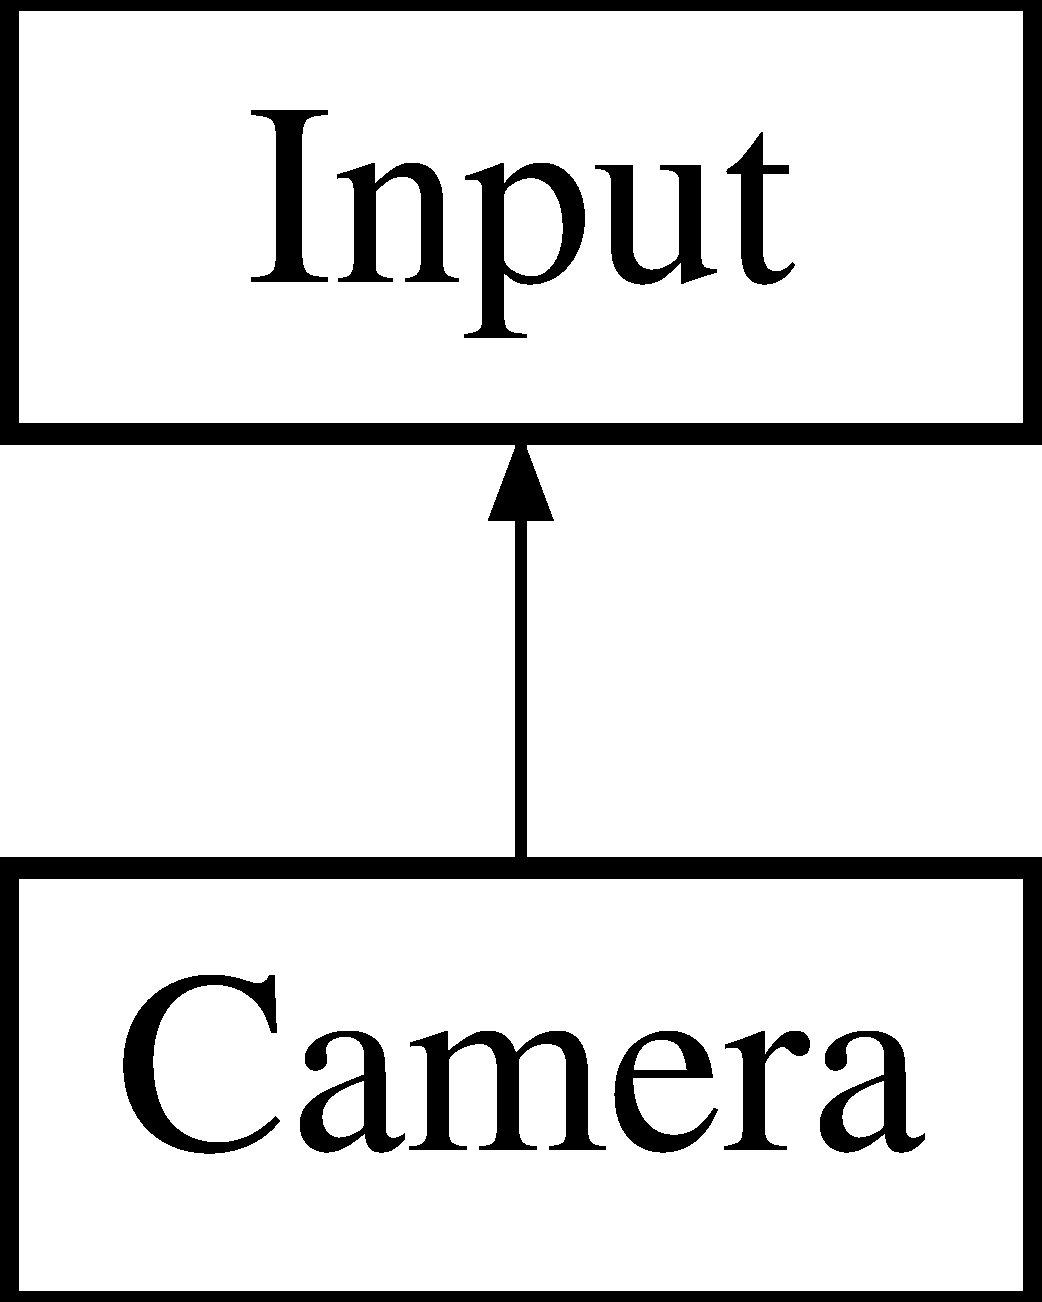
\includegraphics[height=2.000000cm]{class_camera}
\end{center}
\end{figure}
\subsection*{Public Member Functions}
\begin{DoxyCompactItemize}
\item 
\hyperlink{class_camera_a01f94c3543f56ede7af49dc778f19331}{Camera} ()
\item 
void {\bfseries Get\+Eye\+Position} (float \&x, float \&y, float \&z) const \hypertarget{class_camera_a77db484a2cd90ea89a4c42e2ddb50bb9}{}\label{class_camera_a77db484a2cd90ea89a4c42e2ddb50bb9}

\item 
void {\bfseries Get\+View\+Direction} (float \&x, float \&y, float \&z) const \hypertarget{class_camera_a2fb58e261783be389e8f31d72f0e519c}{}\label{class_camera_a2fb58e261783be389e8f31d72f0e519c}

\item 
void {\bfseries Get\+Forward\+Vector} (float \&x, float \&y, float \&z) const \hypertarget{class_camera_a87bb6f576b91e92ae7ab0b40a8b637d0}{}\label{class_camera_a87bb6f576b91e92ae7ab0b40a8b637d0}

\item 
void {\bfseries Get\+Right\+Vector} (float \&x, float \&y, float \&z) const \hypertarget{class_camera_a064623026c61013747babd237b1e4ffb}{}\label{class_camera_a064623026c61013747babd237b1e4ffb}

\item 
void {\bfseries Get\+Up\+Vector} (float \&x, float \&y, float \&z) const \hypertarget{class_camera_ad89f7bc75d6f87de02a252d269d5ba17}{}\label{class_camera_ad89f7bc75d6f87de02a252d269d5ba17}

\item 
void \hyperlink{class_camera_a4502b36b87b9f058bfad2c4716c00c1e}{Update} (const double \&delta\+Time)
\item 
void \hyperlink{class_camera_aa46f58b32270a571ab56dde4caca46db}{Reset} ()
\item 
void \hyperlink{class_camera_a2fea95f244577af436294a9b2c1fd1cc}{Set\+Viewport} ()
\item 
void \hyperlink{class_camera_aafed3cc6d06082a7396c38f4dd4a0549}{Handle\+Key} (unsigned char key, int state, int x, int y)
\item 
void \hyperlink{class_camera_aefce3308a5ed57fbc6666d8935fb7eac}{Handle\+Special\+Key} (int key, int state, int x, int y)
\item 
void \hyperlink{class_camera_adf8b8e5f8f1e88a373f102b3efa12697}{Handle\+Mouse} (int button, int state, int x, int y)
\item 
void \hyperlink{class_camera_af0b7923173a70a13f108ac69a8d9b848}{Handle\+Mouse\+Drag} (int x, int y)
\item 
void \hyperlink{class_camera_a47357f68951777da13bef3234ff7474e}{Handle\+Mouse\+Move} (int x, int y)
\item 
void \hyperlink{class_camera_a62032d7798b96031f332e20e7c8b1794}{Setup\+Camera} ()
\end{DoxyCompactItemize}


\subsection{Detailed Description}
This class implements the base \hyperlink{class_camera}{Camera} functionality. It controls the position and view direction of the camera in your \hyperlink{class_scene}{Scene}. You may add functionality by creating a new class that inherits {\ttfamily \hyperlink{class_camera}{Camera}}, e.\+g.
\begin{DoxyCode}
\textcolor{keyword}{class }MyCamera : \textcolor{keyword}{public} \hyperlink{class_camera}{Camera} 
\end{DoxyCode}
 . You should avoid editting this class directly. 

Note that
\begin{DoxyCode}
\hyperlink{class_camera}{Camera} 
\end{DoxyCode}
 extends the virtual class \hyperlink{class_input}{Input}, so will be passed key and mouse input by the window \begin{DoxyAuthor}{Author}
wil 
\end{DoxyAuthor}


\subsection{Constructor \& Destructor Documentation}
\index{Camera@{Camera}!Camera@{Camera}}
\index{Camera@{Camera}!Camera@{Camera}}
\subsubsection[{\texorpdfstring{Camera()}{Camera()}}]{\setlength{\rightskip}{0pt plus 5cm}Camera\+::\+Camera (
\begin{DoxyParamCaption}
{}
\end{DoxyParamCaption}
)}\hypertarget{class_camera_a01f94c3543f56ede7af49dc778f19331}{}\label{class_camera_a01f94c3543f56ede7af49dc778f19331}
Constructor for \hyperlink{class_camera}{Camera} to set up viewing properties in rendering window 

\subsection{Member Function Documentation}
\index{Camera@{Camera}!Handle\+Key@{Handle\+Key}}
\index{Handle\+Key@{Handle\+Key}!Camera@{Camera}}
\subsubsection[{\texorpdfstring{Handle\+Key(unsigned char key, int state, int x, int y)}{HandleKey(unsigned char key, int state, int x, int y)}}]{\setlength{\rightskip}{0pt plus 5cm}void Camera\+::\+Handle\+Key (
\begin{DoxyParamCaption}
\item[{unsigned char}]{key, }
\item[{int}]{state, }
\item[{int}]{x, }
\item[{int}]{y}
\end{DoxyParamCaption}
)\hspace{0.3cm}{\ttfamily [virtual]}}\hypertarget{class_camera_aafed3cc6d06082a7396c38f4dd4a0549}{}\label{class_camera_aafed3cc6d06082a7396c38f4dd4a0549}
Captures input from
\begin{DoxyCode}
wasd 
\end{DoxyCode}
 -\/keys used for camera movement. 

Spacebar  \#reset() reset\}s the camera. 

Reimplemented from \hyperlink{class_input_a376e4472a9f3621238d6513252949366}{Input}.

\index{Camera@{Camera}!Handle\+Mouse@{Handle\+Mouse}}
\index{Handle\+Mouse@{Handle\+Mouse}!Camera@{Camera}}
\subsubsection[{\texorpdfstring{Handle\+Mouse(int button, int state, int x, int y)}{HandleMouse(int button, int state, int x, int y)}}]{\setlength{\rightskip}{0pt plus 5cm}void Camera\+::\+Handle\+Mouse (
\begin{DoxyParamCaption}
\item[{int}]{button, }
\item[{int}]{state, }
\item[{int}]{x, }
\item[{int}]{y}
\end{DoxyParamCaption}
)\hspace{0.3cm}{\ttfamily [virtual]}}\hypertarget{class_camera_adf8b8e5f8f1e88a373f102b3efa12697}{}\label{class_camera_adf8b8e5f8f1e88a373f102b3efa12697}
Captures button click. Sets button to 0 if last mouse button is released. Saves current position of mouse at click. \begin{DoxySeeAlso}{See also}
\hyperlink{class_camera_af0b7923173a70a13f108ac69a8d9b848}{Handle\+Mouse\+Drag(int, int)} 
\end{DoxySeeAlso}


Reimplemented from \hyperlink{class_input_a85fe43236eb168699ec57b37ab022741}{Input}.

\index{Camera@{Camera}!Handle\+Mouse\+Drag@{Handle\+Mouse\+Drag}}
\index{Handle\+Mouse\+Drag@{Handle\+Mouse\+Drag}!Camera@{Camera}}
\subsubsection[{\texorpdfstring{Handle\+Mouse\+Drag(int x, int y)}{HandleMouseDrag(int x, int y)}}]{\setlength{\rightskip}{0pt plus 5cm}void Camera\+::\+Handle\+Mouse\+Drag (
\begin{DoxyParamCaption}
\item[{int}]{x, }
\item[{int}]{y}
\end{DoxyParamCaption}
)\hspace{0.3cm}{\ttfamily [virtual]}}\hypertarget{class_camera_af0b7923173a70a13f108ac69a8d9b848}{}\label{class_camera_af0b7923173a70a13f108ac69a8d9b848}
Called when mouse is moved (while a button is pressed down). Functionality currently only for {\bfseries L\+E\+FT} mouse click. 

Calculates difference in mouse position since last call and adjusts camera \hyperlink{}{view} accordingly. Sensitivity is fixed at 0.\+01f. \begin{DoxySeeAlso}{See also}
\hyperlink{class_camera_adf8b8e5f8f1e88a373f102b3efa12697}{Handle\+Mouse(int, int, int, int)} 
\end{DoxySeeAlso}


Reimplemented from \hyperlink{class_input_abb590b1b9684b966340a8377ab0d00e2}{Input}.

\index{Camera@{Camera}!Handle\+Mouse\+Move@{Handle\+Mouse\+Move}}
\index{Handle\+Mouse\+Move@{Handle\+Mouse\+Move}!Camera@{Camera}}
\subsubsection[{\texorpdfstring{Handle\+Mouse\+Move(int x, int y)}{HandleMouseMove(int x, int y)}}]{\setlength{\rightskip}{0pt plus 5cm}void Camera\+::\+Handle\+Mouse\+Move (
\begin{DoxyParamCaption}
\item[{int}]{x, }
\item[{int}]{y}
\end{DoxyParamCaption}
)\hspace{0.3cm}{\ttfamily [virtual]}}\hypertarget{class_camera_a47357f68951777da13bef3234ff7474e}{}\label{class_camera_a47357f68951777da13bef3234ff7474e}
Called when mouse is moved in rendering window when no mouse button is pressed \begin{DoxySeeAlso}{See also}
\hyperlink{class_camera_adf8b8e5f8f1e88a373f102b3efa12697}{Handle\+Mouse(int button, int state, int x, int y)} 

\hyperlink{class_camera_af0b7923173a70a13f108ac69a8d9b848}{Handle\+Mouse\+Drag(int x, int y)} 
\end{DoxySeeAlso}

\begin{DoxyParams}{Parameters}
{\em x} & X coordinate of mouse in rendering window \\
\hline
{\em y} & Y coordinate of mouse in rendering window \\
\hline
\end{DoxyParams}


Reimplemented from \hyperlink{class_input_a89177666298fbef2797c677d486bc628}{Input}.

\index{Camera@{Camera}!Handle\+Special\+Key@{Handle\+Special\+Key}}
\index{Handle\+Special\+Key@{Handle\+Special\+Key}!Camera@{Camera}}
\subsubsection[{\texorpdfstring{Handle\+Special\+Key(int key, int state, int x, int y)}{HandleSpecialKey(int key, int state, int x, int y)}}]{\setlength{\rightskip}{0pt plus 5cm}void Camera\+::\+Handle\+Special\+Key (
\begin{DoxyParamCaption}
\item[{int}]{key, }
\item[{int}]{state, }
\item[{int}]{x, }
\item[{int}]{y}
\end{DoxyParamCaption}
)\hspace{0.3cm}{\ttfamily [virtual]}}\hypertarget{class_camera_aefce3308a5ed57fbc6666d8935fb7eac}{}\label{class_camera_aefce3308a5ed57fbc6666d8935fb7eac}
Called when keyboard input is received from special (non-\/\+A\+S\+C\+II) characters. 

key constants are named G\+L\+U\+T\+\_\+\+K\+E\+Y\+\_\+$\ast$ where $\ast$ is the key. For example\+: 

(arrow keys) G\+L\+U\+T\+\_\+\+K\+E\+Y\+\_\+\+UP, G\+L\+U\+T\+\_\+\+K\+E\+Y\+\_\+\+D\+O\+WN, G\+L\+U\+T\+\_\+\+K\+E\+Y\+\_\+\+L\+E\+FT, G\+L\+U\+T\+\_\+\+K\+E\+Y\+\_\+\+R\+I\+G\+HT, 

G\+L\+U\+T\+\_\+\+K\+E\+Y\+\_\+\+P\+A\+G\+E\+\_\+\+UP, G\+L\+U\+T\+\_\+\+K\+E\+Y\+\_\+\+P\+A\+G\+E\+\_\+\+D\+O\+WN, G\+L\+U\+T\+\_\+\+K\+E\+Y\+\_\+\+H\+O\+ME, G\+L\+U\+T\+\_\+\+K\+E\+Y\+\_\+\+E\+ND, 

G\+L\+U\+T\+\_\+\+K\+E\+Y\+\_\+\+F1, G\+L\+U\+T\+\_\+\+K\+E\+Y\+\_\+\+F2, etc. 

Example implementation\+: 
\begin{DoxyCode}
  \textcolor{keywordtype}{void} MyObject::HandleKey(\textcolor{keywordtype}{unsigned} \textcolor{keywordtype}{int} key, \textcolor{keywordtype}{int} state, \textcolor{keywordtype}{int} x, \textcolor{keywordtype}{int} y)\{
      \textcolor{keywordflow}{if} (state == 1)\{ \textcolor{comment}{// if key pressed down}
        \textcolor{keywordflow}{switch}(key)\{ \textcolor{comment}{// special key}
            \textcolor{keywordflow}{case} GLUT\_KEY\_LEFT:
                  glTranslate(-1.f,0.f,0.f); \textcolor{comment}{// go left}
                \textcolor{keywordflow}{break};
            \textcolor{keywordflow}{case} GLUT\_KEY\_RIGHT:
                  glTranslate(1.f,0.f,0.f); \textcolor{comment}{// go right}
                \textcolor{keywordflow}{break};
        \}
    \}
\}
\end{DoxyCode}
 \begin{DoxySeeAlso}{See also}
\#\+Handle\+Key(char key, int state, int x, int y) 
\end{DoxySeeAlso}

\begin{DoxyParams}{Parameters}
{\em key} & coded keyboard input \\
\hline
{\em state} & 1 if key down, 0 if key up \\
\hline
{\em x} & X coordinate of mouse in rendering window \\
\hline
{\em y} & Y coordinate of mouse in rendering window \\
\hline
\end{DoxyParams}


Reimplemented from \hyperlink{class_input_adccce536f10dfe4b1de2bb22ed8ae538}{Input}.

\index{Camera@{Camera}!Reset@{Reset}}
\index{Reset@{Reset}!Camera@{Camera}}
\subsubsection[{\texorpdfstring{Reset()}{Reset()}}]{\setlength{\rightskip}{0pt plus 5cm}void Camera\+::\+Reset (
\begin{DoxyParamCaption}
{}
\end{DoxyParamCaption}
)}\hypertarget{class_camera_aa46f58b32270a571ab56dde4caca46db}{}\label{class_camera_aa46f58b32270a571ab56dde4caca46db}
Resets \hyperlink{class_camera}{Camera} vectors to default values. Sets position of camera at (0,0) in x,y-\/plane and puts z-\/position at
\begin{DoxyCode}
0.5*height/tan(pi/6) 
\end{DoxyCode}
 which puts the coordinate width and height of window into view (if projection is in perspective view, and both
\begin{DoxyCode}
fovy = 60 
\end{DoxyCode}
 \textdegree{} and
\begin{DoxyCode}
aspect =  width/height 
\end{DoxyCode}
 ) 


\begin{DoxyCode}
width 
\end{DoxyCode}
 and
\begin{DoxyCode}
height 
\end{DoxyCode}
 refer to the window size of
\begin{DoxyCode}
\hyperlink{class_scene}{Scene} 
\end{DoxyCode}
 \hyperlink{}{parent}. \index{Camera@{Camera}!Setup\+Camera@{Setup\+Camera}}
\index{Setup\+Camera@{Setup\+Camera}!Camera@{Camera}}
\subsubsection[{\texorpdfstring{Setup\+Camera()}{SetupCamera()}}]{\setlength{\rightskip}{0pt plus 5cm}void Camera\+::\+Setup\+Camera (
\begin{DoxyParamCaption}
{}
\end{DoxyParamCaption}
)}\hypertarget{class_camera_a62032d7798b96031f332e20e7c8b1794}{}\label{class_camera_a62032d7798b96031f332e20e7c8b1794}
Called by \hyperlink{class_scene}{Scene} to position camera. 

Sets up position (\hyperlink{}{eye}), look at (
\begin{DoxyCode}
cen= 
\end{DoxyCode}
 \hyperlink{}{eye}
\begin{DoxyCode}
+ 
\end{DoxyCode}
 \hyperlink{}{view}) and up vector (\hyperlink{}{up}) and updates \hyperlink{class_scene}{Scene} viewing. \begin{DoxySeeAlso}{See also}
\#\+Update(float) 

\hyperlink{class_camera_aa46f58b32270a571ab56dde4caca46db}{Reset()} 
\end{DoxySeeAlso}
\index{Camera@{Camera}!Set\+Viewport@{Set\+Viewport}}
\index{Set\+Viewport@{Set\+Viewport}!Camera@{Camera}}
\subsubsection[{\texorpdfstring{Set\+Viewport()}{SetViewport()}}]{\setlength{\rightskip}{0pt plus 5cm}void Camera\+::\+Set\+Viewport (
\begin{DoxyParamCaption}
{}
\end{DoxyParamCaption}
)}\hypertarget{class_camera_a2fea95f244577af436294a9b2c1fd1cc}{}\label{class_camera_a2fea95f244577af436294a9b2c1fd1cc}
Sets the window viewport of the scene \index{Camera@{Camera}!Update@{Update}}
\index{Update@{Update}!Camera@{Camera}}
\subsubsection[{\texorpdfstring{Update(const double \&delta\+Time)}{Update(const double &deltaTime)}}]{\setlength{\rightskip}{0pt plus 5cm}void Camera\+::\+Update (
\begin{DoxyParamCaption}
\item[{const double \&}]{delta\+Time}
\end{DoxyParamCaption}
)}\hypertarget{class_camera_a4502b36b87b9f058bfad2c4716c00c1e}{}\label{class_camera_a4502b36b87b9f058bfad2c4716c00c1e}
Update the position of the camera and look-\/at vectors based on keyboard input. 
\begin{DoxyParams}{Parameters}
{\em delta\+Time} & change in time since previous call (unused) \\
\hline
\end{DoxyParams}


The documentation for this class was generated from the following files\+:\begin{DoxyCompactItemize}
\item 
Framework/\+Utility/Camera.\+h\item 
Framework/\+Utility/Camera.\+cpp\end{DoxyCompactItemize}

\hypertarget{class_displayable_object}{}\section{Displayable\+Object Class Reference}
\label{class_displayable_object}\index{Displayable\+Object@{Displayable\+Object}}


{\ttfamily \#include $<$Displayable\+Object.\+h$>$}

\subsection*{Public Member Functions}
\begin{DoxyCompactItemize}
\item 
\hyperlink{class_displayable_object_a2de32e213b8b7f16e72f385e8bf3c7e8}{Displayable\+Object} ()
\item 
virtual void \hyperlink{class_displayable_object_af1fe25dbf6950d41cbf9b99277d0d825}{Display} ()=0
\item 
void \hyperlink{class_displayable_object_afe2221908b0bf6746ae39d15a3422627}{position} (float x, float y, float z)
\item 
void \hyperlink{class_displayable_object_ae5da1215619f8119a2fa9b79bbc52534}{size} (float s)
\item 
void \hyperlink{class_displayable_object_ac199796e336d20345eabd48c5a8d559f}{size} (float sx, float sy, float sz)
\item 
void \hyperlink{class_displayable_object_a0101b77de7909105221c772e8b969d48}{orientation} (float rx, float ry, float rz)
\item 
float $\ast$ \hyperlink{class_displayable_object_ab321394a5a8fab049f6092051d0183cc}{size} ()
\item 
float $\ast$ \hyperlink{class_displayable_object_ac2bf3fd3c6e8c902e250c9df4b06dc1b}{orientation} ()
\item 
float $\ast$ \hyperlink{class_displayable_object_a5c50e13b8274882a8dcfe2582bb9c5df}{position} ()
\end{DoxyCompactItemize}
\subsection*{Protected Attributes}
\begin{DoxyCompactItemize}
\item 
float \hyperlink{class_displayable_object_a7cc44f282422020c02184f34861b6f7a}{pos} \mbox{[}3\mbox{]}
\item 
float \hyperlink{class_displayable_object_aedc1ec03b36a5be1b5ff6c27a361c6f6}{scale} \mbox{[}3\mbox{]}
\item 
float \hyperlink{class_displayable_object_a9f828c99272a0de1910c6ffb19b0f7d1}{rotation} \mbox{[}3\mbox{]}
\end{DoxyCompactItemize}


\subsection{Detailed Description}
Virtual class to be inherited by all objects to be displayed in \hyperlink{class_scene}{Scene} 

Contains purely virtual \hyperlink{class_displayable_object_af1fe25dbf6950d41cbf9b99277d0d825}{Display} method that must be overloaded. \hyperlink{class_displayable_object_af1fe25dbf6950d41cbf9b99277d0d825}{Display()} is called from \hyperlink{class_scene}{Scene}. \begin{DoxyAuthor}{Author}
wil 
\end{DoxyAuthor}


\subsection{Constructor \& Destructor Documentation}
\index{Displayable\+Object@{Displayable\+Object}!Displayable\+Object@{Displayable\+Object}}
\index{Displayable\+Object@{Displayable\+Object}!Displayable\+Object@{Displayable\+Object}}
\subsubsection[{\texorpdfstring{Displayable\+Object()}{DisplayableObject()}}]{\setlength{\rightskip}{0pt plus 5cm}Displayable\+Object\+::\+Displayable\+Object (
\begin{DoxyParamCaption}
{}
\end{DoxyParamCaption}
)\hspace{0.3cm}{\ttfamily [inline]}}\hypertarget{class_displayable_object_a2de32e213b8b7f16e72f385e8bf3c7e8}{}\label{class_displayable_object_a2de32e213b8b7f16e72f385e8bf3c7e8}
Default constructor 

Initialises position, size and orientation to origin in World Space. 

\subsection{Member Function Documentation}
\index{Displayable\+Object@{Displayable\+Object}!Display@{Display}}
\index{Display@{Display}!Displayable\+Object@{Displayable\+Object}}
\subsubsection[{\texorpdfstring{Display()=0}{Display()=0}}]{\setlength{\rightskip}{0pt plus 5cm}virtual void Displayable\+Object\+::\+Display (
\begin{DoxyParamCaption}
{}
\end{DoxyParamCaption}
)\hspace{0.3cm}{\ttfamily [pure virtual]}}\hypertarget{class_displayable_object_af1fe25dbf6950d41cbf9b99277d0d825}{}\label{class_displayable_object_af1fe25dbf6950d41cbf9b99277d0d825}
Virtual method. Called from \hyperlink{class_scene}{Scene} parent. 

Must be overloaded by your \hyperlink{class_displayable_object}{Displayable\+Object} subclass. Contains all rendering commands. \index{Displayable\+Object@{Displayable\+Object}!orientation@{orientation}}
\index{orientation@{orientation}!Displayable\+Object@{Displayable\+Object}}
\subsubsection[{\texorpdfstring{orientation(float rx, float ry, float rz)}{orientation(float rx, float ry, float rz)}}]{\setlength{\rightskip}{0pt plus 5cm}void Displayable\+Object\+::orientation (
\begin{DoxyParamCaption}
\item[{float}]{rx, }
\item[{float}]{ry, }
\item[{float}]{rz}
\end{DoxyParamCaption}
)\hspace{0.3cm}{\ttfamily [inline]}}\hypertarget{class_displayable_object_a0101b77de7909105221c772e8b969d48}{}\label{class_displayable_object_a0101b77de7909105221c772e8b969d48}
set orientation in World Space \index{Displayable\+Object@{Displayable\+Object}!orientation@{orientation}}
\index{orientation@{orientation}!Displayable\+Object@{Displayable\+Object}}
\subsubsection[{\texorpdfstring{orientation()}{orientation()}}]{\setlength{\rightskip}{0pt plus 5cm}float$\ast$ Displayable\+Object\+::orientation (
\begin{DoxyParamCaption}
{}
\end{DoxyParamCaption}
)\hspace{0.3cm}{\ttfamily [inline]}}\hypertarget{class_displayable_object_ac2bf3fd3c6e8c902e250c9df4b06dc1b}{}\label{class_displayable_object_ac2bf3fd3c6e8c902e250c9df4b06dc1b}
Get orientation in World Space \index{Displayable\+Object@{Displayable\+Object}!position@{position}}
\index{position@{position}!Displayable\+Object@{Displayable\+Object}}
\subsubsection[{\texorpdfstring{position(float x, float y, float z)}{position(float x, float y, float z)}}]{\setlength{\rightskip}{0pt plus 5cm}void Displayable\+Object\+::position (
\begin{DoxyParamCaption}
\item[{float}]{x, }
\item[{float}]{y, }
\item[{float}]{z}
\end{DoxyParamCaption}
)\hspace{0.3cm}{\ttfamily [inline]}}\hypertarget{class_displayable_object_afe2221908b0bf6746ae39d15a3422627}{}\label{class_displayable_object_afe2221908b0bf6746ae39d15a3422627}
set World Space position \index{Displayable\+Object@{Displayable\+Object}!position@{position}}
\index{position@{position}!Displayable\+Object@{Displayable\+Object}}
\subsubsection[{\texorpdfstring{position()}{position()}}]{\setlength{\rightskip}{0pt plus 5cm}float$\ast$ Displayable\+Object\+::position (
\begin{DoxyParamCaption}
{}
\end{DoxyParamCaption}
)\hspace{0.3cm}{\ttfamily [inline]}}\hypertarget{class_displayable_object_a5c50e13b8274882a8dcfe2582bb9c5df}{}\label{class_displayable_object_a5c50e13b8274882a8dcfe2582bb9c5df}
Get World Space position \index{Displayable\+Object@{Displayable\+Object}!size@{size}}
\index{size@{size}!Displayable\+Object@{Displayable\+Object}}
\subsubsection[{\texorpdfstring{size(float s)}{size(float s)}}]{\setlength{\rightskip}{0pt plus 5cm}void Displayable\+Object\+::size (
\begin{DoxyParamCaption}
\item[{float}]{s}
\end{DoxyParamCaption}
)\hspace{0.3cm}{\ttfamily [inline]}}\hypertarget{class_displayable_object_ae5da1215619f8119a2fa9b79bbc52534}{}\label{class_displayable_object_ae5da1215619f8119a2fa9b79bbc52534}
set size in World Space (single value) \index{Displayable\+Object@{Displayable\+Object}!size@{size}}
\index{size@{size}!Displayable\+Object@{Displayable\+Object}}
\subsubsection[{\texorpdfstring{size(float sx, float sy, float sz)}{size(float sx, float sy, float sz)}}]{\setlength{\rightskip}{0pt plus 5cm}void Displayable\+Object\+::size (
\begin{DoxyParamCaption}
\item[{float}]{sx, }
\item[{float}]{sy, }
\item[{float}]{sz}
\end{DoxyParamCaption}
)\hspace{0.3cm}{\ttfamily [inline]}}\hypertarget{class_displayable_object_ac199796e336d20345eabd48c5a8d559f}{}\label{class_displayable_object_ac199796e336d20345eabd48c5a8d559f}
set size in World Space (seperate axes) \index{Displayable\+Object@{Displayable\+Object}!size@{size}}
\index{size@{size}!Displayable\+Object@{Displayable\+Object}}
\subsubsection[{\texorpdfstring{size()}{size()}}]{\setlength{\rightskip}{0pt plus 5cm}float$\ast$ Displayable\+Object\+::size (
\begin{DoxyParamCaption}
{}
\end{DoxyParamCaption}
)\hspace{0.3cm}{\ttfamily [inline]}}\hypertarget{class_displayable_object_ab321394a5a8fab049f6092051d0183cc}{}\label{class_displayable_object_ab321394a5a8fab049f6092051d0183cc}
Get size in World Space 

\subsection{Member Data Documentation}
\index{Displayable\+Object@{Displayable\+Object}!pos@{pos}}
\index{pos@{pos}!Displayable\+Object@{Displayable\+Object}}
\subsubsection[{\texorpdfstring{pos}{pos}}]{\setlength{\rightskip}{0pt plus 5cm}float Displayable\+Object\+::pos\mbox{[}3\mbox{]}\hspace{0.3cm}{\ttfamily [protected]}}\hypertarget{class_displayable_object_a7cc44f282422020c02184f34861b6f7a}{}\label{class_displayable_object_a7cc44f282422020c02184f34861b6f7a}
float\mbox{[}\mbox{]} containing World Space position coordinates \index{Displayable\+Object@{Displayable\+Object}!rotation@{rotation}}
\index{rotation@{rotation}!Displayable\+Object@{Displayable\+Object}}
\subsubsection[{\texorpdfstring{rotation}{rotation}}]{\setlength{\rightskip}{0pt plus 5cm}float Displayable\+Object\+::rotation\mbox{[}3\mbox{]}\hspace{0.3cm}{\ttfamily [protected]}}\hypertarget{class_displayable_object_a9f828c99272a0de1910c6ffb19b0f7d1}{}\label{class_displayable_object_a9f828c99272a0de1910c6ffb19b0f7d1}
float\mbox{[}\mbox{]} containing angles of orientation in World Space for x, y, and z axes \index{Displayable\+Object@{Displayable\+Object}!scale@{scale}}
\index{scale@{scale}!Displayable\+Object@{Displayable\+Object}}
\subsubsection[{\texorpdfstring{scale}{scale}}]{\setlength{\rightskip}{0pt plus 5cm}float Displayable\+Object\+::scale\mbox{[}3\mbox{]}\hspace{0.3cm}{\ttfamily [protected]}}\hypertarget{class_displayable_object_aedc1ec03b36a5be1b5ff6c27a361c6f6}{}\label{class_displayable_object_aedc1ec03b36a5be1b5ff6c27a361c6f6}
float\mbox{[}\mbox{]} containing relative World Space scaling values for x,y,z 

The documentation for this class was generated from the following file\+:\begin{DoxyCompactItemize}
\item 
Framework/\+Interface/Displayable\+Object.\+h\end{DoxyCompactItemize}

\hypertarget{class_engine}{}\section{Engine Class Reference}
\label{class_engine}\index{Engine@{Engine}}


{\ttfamily \#include $<$Engine.\+h$>$}

Inheritance diagram for Engine\+:\begin{figure}[H]
\begin{center}
\leavevmode
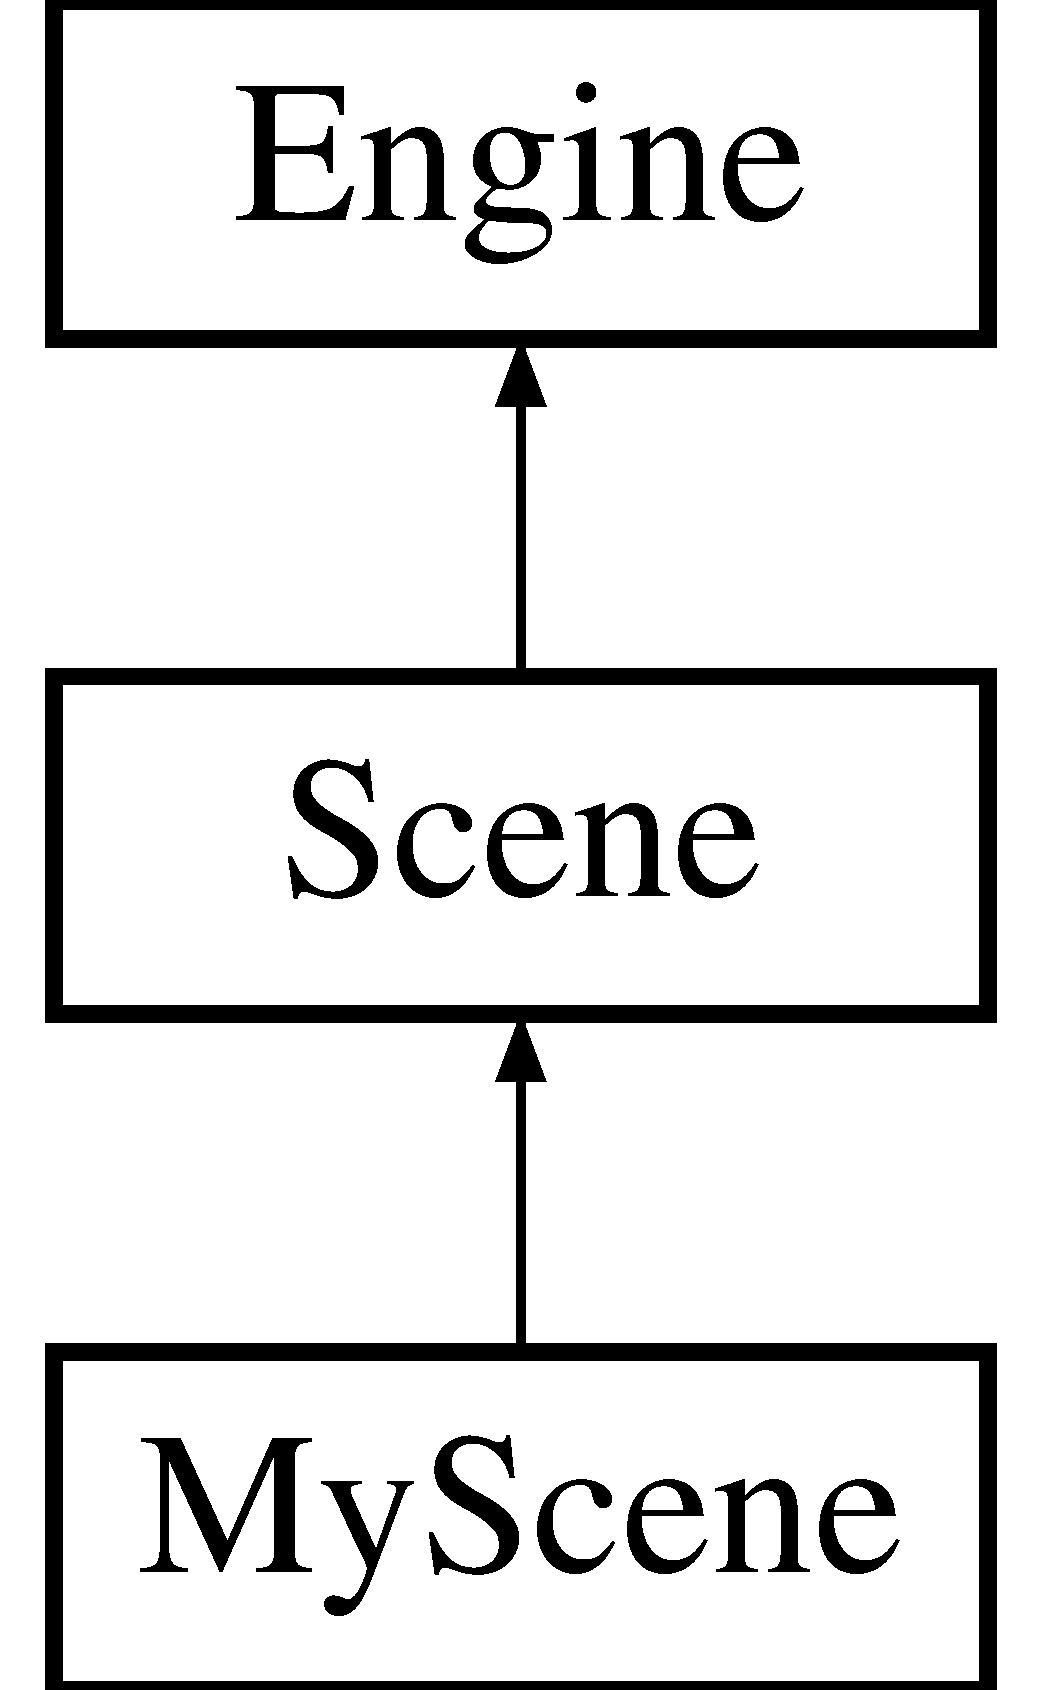
\includegraphics[height=3.000000cm]{class_engine}
\end{center}
\end{figure}
\subsection*{Public Member Functions}
\begin{DoxyCompactItemize}
\item 
\hyperlink{class_engine_a06d6fce9529416545e9b88edf5128358}{Engine} (int argc, char $\ast$$\ast$argv, const char $\ast$title, const int \&window\+Width, const int \&window\+Height)
\item 
virtual void \hyperlink{class_engine_af4c789fb939a0870426c698a5124a0ee}{Run} ()
\end{DoxyCompactItemize}
\subsection*{Static Public Member Functions}
\begin{DoxyCompactItemize}
\item 
static \hyperlink{class_engine}{Engine} $\ast$ \hyperlink{class_engine_ae9f9fcca9bc01336382a0d49fed6d160}{Get\+Current\+Instance} ()
\item 
static const char $\ast$ \hyperlink{class_engine_ae87b850ce1f35b1b19bdefa0bfc598a8}{Get\+Window\+Title} ()
\item 
static int \hyperlink{class_engine_ae7020ad5026116cbbc1d89a67c41a5af}{Get\+Window\+ID} ()
\item 
static int \hyperlink{class_engine_afe21f271a38196c447d364a68c3ba00a}{Get\+Window\+Width} ()
\item 
static int \hyperlink{class_engine_af3d49b062bf02821155f5e5b563c245d}{Get\+Window\+Height} ()
\end{DoxyCompactItemize}
\subsection*{Protected Member Functions}
\begin{DoxyCompactItemize}
\item 
virtual void {\bfseries Initialise} ()=0\hypertarget{class_engine_a43a803fae8d4672c9119763c438825ad}{}\label{class_engine_a43a803fae8d4672c9119763c438825ad}

\item 
virtual void {\bfseries Draw} ()=0\hypertarget{class_engine_abc33391595849f65f99eb5f145535b72}{}\label{class_engine_abc33391595849f65f99eb5f145535b72}

\item 
virtual void {\bfseries Reshape} (int w, int h)=0\hypertarget{class_engine_a8c958c38482fbc3e2dfc3d7f2515d2c1}{}\label{class_engine_a8c958c38482fbc3e2dfc3d7f2515d2c1}

\item 
virtual void {\bfseries Update} (const double \&)=0\hypertarget{class_engine_a258aff43face90f1a4911b2c30cb5c58}{}\label{class_engine_a258aff43face90f1a4911b2c30cb5c58}

\item 
virtual void {\bfseries Handle\+Key} (unsigned char key, int state, int x, int y)=0\hypertarget{class_engine_ae64af2ed4a8c6629a7aa7254a0fd892a}{}\label{class_engine_ae64af2ed4a8c6629a7aa7254a0fd892a}

\item 
virtual void {\bfseries Handle\+Special\+Key} (int key, int state, int x, int y)=0\hypertarget{class_engine_ade235e5c6e7b67660205143235b8b918}{}\label{class_engine_ade235e5c6e7b67660205143235b8b918}

\item 
virtual void {\bfseries Handle\+Mouse} (int button, int state, int x, int y)=0\hypertarget{class_engine_a26cd386d9286261e9aadbcf8082110ca}{}\label{class_engine_a26cd386d9286261e9aadbcf8082110ca}

\item 
virtual void {\bfseries Handle\+Mouse\+Drag} (int x, int y)=0\hypertarget{class_engine_a88faed8e9d03f3e734ba328c962c0d95}{}\label{class_engine_a88faed8e9d03f3e734ba328c962c0d95}

\item 
virtual void {\bfseries Handle\+Mouse\+Move} (int x, int y)=0\hypertarget{class_engine_aec49b2c8ad382a7ca5f5998fbe4d995b}{}\label{class_engine_aec49b2c8ad382a7ca5f5998fbe4d995b}

\end{DoxyCompactItemize}
\subsection*{Static Protected Member Functions}
\begin{DoxyCompactItemize}
\item 
static void \hyperlink{class_engine_abe5871e891fe327f17cb8bf28693e45d}{Init\+Func} ()
\item 
static void \hyperlink{class_engine_a0e5ef99e1d81785bd157634a9fe583ce}{Draw\+Func} ()
\item 
static void \hyperlink{class_engine_a5a05897a147382a9d271c8dbd262b4a5}{Idle\+Func} ()
\item 
static void \hyperlink{class_engine_abbc06815bf06ce7d560c1965067fa2e7}{Resize\+Func} (int \+\_\+width, int \+\_\+height)
\item 
static void \hyperlink{class_engine_ae201229f027168e251abc776d2e9a2e0}{Key\+Down\+Func} (unsigned char key, int x, int y)
\item 
static void \hyperlink{class_engine_a3f2e2df3c913b773cc185d21860da5d6}{Key\+Up\+Func} (unsigned char key, int x, int y)
\item 
static void \hyperlink{class_engine_ac21b173d6d9ec44c363989c3666061f5}{Special\+Key\+Down\+Func} (int key, int x, int y)
\item 
static void \hyperlink{class_engine_a0c66abbd2cfd67a99943d65f64a7951d}{Special\+Key\+Up\+Func} (int key, int x, int y)
\item 
static void \hyperlink{class_engine_ad016f923c1e398e192caed6e5ca9d66b}{Mouse\+Func} (int button, int state, int x, int y)
\item 
static void \hyperlink{class_engine_a163556fac75da746d32a4e776ca1461b}{Mouse\+Motion\+Func} (int x, int y)
\item 
static void \hyperlink{class_engine_a85c184fddc04c11711d7d257bb5e7954}{Passive\+Mouse\+Motion\+Func} (int x, int y)
\item 
static int \hyperlink{class_engine_ab6b8b85aa27ec75c3a0b61c38453c372}{Check\+G\+L\+Error} ()
\end{DoxyCompactItemize}
\subsection*{Static Protected Attributes}
\begin{DoxyCompactItemize}
\item 
static \hyperlink{class_engine}{Engine} $\ast$ \hyperlink{class_engine_a74455645fff2e37cf3f6ad65a0709b3e}{current} = 0
\item 
static const char $\ast$ {\bfseries window\+Title} = \char`\"{}\char`\"{}\hypertarget{class_engine_afbe66082c7f1794516bff6e963e630b7}{}\label{class_engine_afbe66082c7f1794516bff6e963e630b7}

\item 
static int {\bfseries window\+ID} = 0\hypertarget{class_engine_a8319283c604ee6fce0cacae8fbd3ed33}{}\label{class_engine_a8319283c604ee6fce0cacae8fbd3ed33}

\item 
static int {\bfseries window\+Width} = 0\hypertarget{class_engine_a541d921b6b97e8756522958a58814344}{}\label{class_engine_a541d921b6b97e8756522958a58814344}

\item 
static int {\bfseries window\+Height} = 0\hypertarget{class_engine_a0ac480c63e98dd9b1fe4c4a3c9e6a7ca}{}\label{class_engine_a0ac480c63e98dd9b1fe4c4a3c9e6a7ca}

\item 
static int {\bfseries time} = 0\hypertarget{class_engine_a0c18d7f954663e37f58ed6f06c7040e0}{}\label{class_engine_a0c18d7f954663e37f58ed6f06c7040e0}

\end{DoxyCompactItemize}


\subsection{Detailed Description}
Base \hyperlink{class_engine}{Engine} for the framework. Handles windowing and freeglut/\+Open\+GL contexts. \hyperlink{class_engine}{Engine} is static. 

\subsection{Constructor \& Destructor Documentation}
\index{Engine@{Engine}!Engine@{Engine}}
\index{Engine@{Engine}!Engine@{Engine}}
\subsubsection[{\texorpdfstring{Engine(int argc, char $\ast$$\ast$argv, const char $\ast$title, const int \&window\+Width, const int \&window\+Height)}{Engine(int argc, char **argv, const char *title, const int &windowWidth, const int &windowHeight)}}]{\setlength{\rightskip}{0pt plus 5cm}Engine\+::\+Engine (
\begin{DoxyParamCaption}
\item[{int}]{argc, }
\item[{char $\ast$$\ast$}]{argv, }
\item[{const char $\ast$}]{title, }
\item[{const int \&}]{window\+Width, }
\item[{const int \&}]{window\+Height}
\end{DoxyParamCaption}
)}\hypertarget{class_engine_a06d6fce9529416545e9b88edf5128358}{}\label{class_engine_a06d6fce9529416545e9b88edf5128358}
Constructor takes in command line arguments, a title and initial window dimensions. 

\subsection{Member Function Documentation}
\index{Engine@{Engine}!Check\+G\+L\+Error@{Check\+G\+L\+Error}}
\index{Check\+G\+L\+Error@{Check\+G\+L\+Error}!Engine@{Engine}}
\subsubsection[{\texorpdfstring{Check\+G\+L\+Error()}{CheckGLError()}}]{\setlength{\rightskip}{0pt plus 5cm}int Engine\+::\+Check\+G\+L\+Error (
\begin{DoxyParamCaption}
{}
\end{DoxyParamCaption}
)\hspace{0.3cm}{\ttfamily [static]}, {\ttfamily [protected]}}\hypertarget{class_engine_ab6b8b85aa27ec75c3a0b61c38453c372}{}\label{class_engine_ab6b8b85aa27ec75c3a0b61c38453c372}
Iterates through Open\+GL error list and dumps error information to console. 

Call this method in a draw loop. \index{Engine@{Engine}!Draw\+Func@{Draw\+Func}}
\index{Draw\+Func@{Draw\+Func}!Engine@{Engine}}
\subsubsection[{\texorpdfstring{Draw\+Func()}{DrawFunc()}}]{\setlength{\rightskip}{0pt plus 5cm}void Engine\+::\+Draw\+Func (
\begin{DoxyParamCaption}
{}
\end{DoxyParamCaption}
)\hspace{0.3cm}{\ttfamily [static]}, {\ttfamily [protected]}}\hypertarget{class_engine_a0e5ef99e1d81785bd157634a9fe583ce}{}\label{class_engine_a0e5ef99e1d81785bd157634a9fe583ce}
Calls \hyperlink{}{Draw} and handles double buffering \index{Engine@{Engine}!Get\+Current\+Instance@{Get\+Current\+Instance}}
\index{Get\+Current\+Instance@{Get\+Current\+Instance}!Engine@{Engine}}
\subsubsection[{\texorpdfstring{Get\+Current\+Instance()}{GetCurrentInstance()}}]{\setlength{\rightskip}{0pt plus 5cm}{\bf Engine} $\ast$ Engine\+::\+Get\+Current\+Instance (
\begin{DoxyParamCaption}
{}
\end{DoxyParamCaption}
)\hspace{0.3cm}{\ttfamily [static]}}\hypertarget{class_engine_ae9f9fcca9bc01336382a0d49fed6d160}{}\label{class_engine_ae9f9fcca9bc01336382a0d49fed6d160}
Returns self. \index{Engine@{Engine}!Get\+Window\+Height@{Get\+Window\+Height}}
\index{Get\+Window\+Height@{Get\+Window\+Height}!Engine@{Engine}}
\subsubsection[{\texorpdfstring{Get\+Window\+Height()}{GetWindowHeight()}}]{\setlength{\rightskip}{0pt plus 5cm}int Engine\+::\+Get\+Window\+Height (
\begin{DoxyParamCaption}
{}
\end{DoxyParamCaption}
)\hspace{0.3cm}{\ttfamily [static]}}\hypertarget{class_engine_af3d49b062bf02821155f5e5b563c245d}{}\label{class_engine_af3d49b062bf02821155f5e5b563c245d}
Returns window height \index{Engine@{Engine}!Get\+Window\+ID@{Get\+Window\+ID}}
\index{Get\+Window\+ID@{Get\+Window\+ID}!Engine@{Engine}}
\subsubsection[{\texorpdfstring{Get\+Window\+I\+D()}{GetWindowID()}}]{\setlength{\rightskip}{0pt plus 5cm}int Engine\+::\+Get\+Window\+ID (
\begin{DoxyParamCaption}
{}
\end{DoxyParamCaption}
)\hspace{0.3cm}{\ttfamily [static]}}\hypertarget{class_engine_ae7020ad5026116cbbc1d89a67c41a5af}{}\label{class_engine_ae7020ad5026116cbbc1d89a67c41a5af}
Returns window id \index{Engine@{Engine}!Get\+Window\+Title@{Get\+Window\+Title}}
\index{Get\+Window\+Title@{Get\+Window\+Title}!Engine@{Engine}}
\subsubsection[{\texorpdfstring{Get\+Window\+Title()}{GetWindowTitle()}}]{\setlength{\rightskip}{0pt plus 5cm}const char $\ast$ Engine\+::\+Get\+Window\+Title (
\begin{DoxyParamCaption}
{}
\end{DoxyParamCaption}
)\hspace{0.3cm}{\ttfamily [static]}}\hypertarget{class_engine_ae87b850ce1f35b1b19bdefa0bfc598a8}{}\label{class_engine_ae87b850ce1f35b1b19bdefa0bfc598a8}
Returns window title \index{Engine@{Engine}!Get\+Window\+Width@{Get\+Window\+Width}}
\index{Get\+Window\+Width@{Get\+Window\+Width}!Engine@{Engine}}
\subsubsection[{\texorpdfstring{Get\+Window\+Width()}{GetWindowWidth()}}]{\setlength{\rightskip}{0pt plus 5cm}int Engine\+::\+Get\+Window\+Width (
\begin{DoxyParamCaption}
{}
\end{DoxyParamCaption}
)\hspace{0.3cm}{\ttfamily [static]}}\hypertarget{class_engine_afe21f271a38196c447d364a68c3ba00a}{}\label{class_engine_afe21f271a38196c447d364a68c3ba00a}
Returns window width \index{Engine@{Engine}!Idle\+Func@{Idle\+Func}}
\index{Idle\+Func@{Idle\+Func}!Engine@{Engine}}
\subsubsection[{\texorpdfstring{Idle\+Func()}{IdleFunc()}}]{\setlength{\rightskip}{0pt plus 5cm}void Engine\+::\+Idle\+Func (
\begin{DoxyParamCaption}
{}
\end{DoxyParamCaption}
)\hspace{0.3cm}{\ttfamily [static]}, {\ttfamily [protected]}}\hypertarget{class_engine_a5a05897a147382a9d271c8dbd262b4a5}{}\label{class_engine_a5a05897a147382a9d271c8dbd262b4a5}
Checks runtime between successive calls and runs \hyperlink{}{Update} before pushing redisplay \index{Engine@{Engine}!Init\+Func@{Init\+Func}}
\index{Init\+Func@{Init\+Func}!Engine@{Engine}}
\subsubsection[{\texorpdfstring{Init\+Func()}{InitFunc()}}]{\setlength{\rightskip}{0pt plus 5cm}void Engine\+::\+Init\+Func (
\begin{DoxyParamCaption}
{}
\end{DoxyParamCaption}
)\hspace{0.3cm}{\ttfamily [static]}, {\ttfamily [protected]}}\hypertarget{class_engine_abe5871e891fe327f17cb8bf28693e45d}{}\label{class_engine_abe5871e891fe327f17cb8bf28693e45d}
Sets up default initial functionality for window \index{Engine@{Engine}!Key\+Down\+Func@{Key\+Down\+Func}}
\index{Key\+Down\+Func@{Key\+Down\+Func}!Engine@{Engine}}
\subsubsection[{\texorpdfstring{Key\+Down\+Func(unsigned char key, int x, int y)}{KeyDownFunc(unsigned char key, int x, int y)}}]{\setlength{\rightskip}{0pt plus 5cm}void Engine\+::\+Key\+Down\+Func (
\begin{DoxyParamCaption}
\item[{unsigned char}]{key, }
\item[{int}]{x, }
\item[{int}]{y}
\end{DoxyParamCaption}
)\hspace{0.3cm}{\ttfamily [static]}, {\ttfamily [protected]}}\hypertarget{class_engine_ae201229f027168e251abc776d2e9a2e0}{}\label{class_engine_ae201229f027168e251abc776d2e9a2e0}
Handles key press \index{Engine@{Engine}!Key\+Up\+Func@{Key\+Up\+Func}}
\index{Key\+Up\+Func@{Key\+Up\+Func}!Engine@{Engine}}
\subsubsection[{\texorpdfstring{Key\+Up\+Func(unsigned char key, int x, int y)}{KeyUpFunc(unsigned char key, int x, int y)}}]{\setlength{\rightskip}{0pt plus 5cm}void Engine\+::\+Key\+Up\+Func (
\begin{DoxyParamCaption}
\item[{unsigned char}]{key, }
\item[{int}]{x, }
\item[{int}]{y}
\end{DoxyParamCaption}
)\hspace{0.3cm}{\ttfamily [static]}, {\ttfamily [protected]}}\hypertarget{class_engine_a3f2e2df3c913b773cc185d21860da5d6}{}\label{class_engine_a3f2e2df3c913b773cc185d21860da5d6}
Handles key release \index{Engine@{Engine}!Mouse\+Func@{Mouse\+Func}}
\index{Mouse\+Func@{Mouse\+Func}!Engine@{Engine}}
\subsubsection[{\texorpdfstring{Mouse\+Func(int button, int state, int x, int y)}{MouseFunc(int button, int state, int x, int y)}}]{\setlength{\rightskip}{0pt plus 5cm}void Engine\+::\+Mouse\+Func (
\begin{DoxyParamCaption}
\item[{int}]{button, }
\item[{int}]{state, }
\item[{int}]{x, }
\item[{int}]{y}
\end{DoxyParamCaption}
)\hspace{0.3cm}{\ttfamily [static]}, {\ttfamily [protected]}}\hypertarget{class_engine_ad016f923c1e398e192caed6e5ca9d66b}{}\label{class_engine_ad016f923c1e398e192caed6e5ca9d66b}
Handles mouse button click \index{Engine@{Engine}!Mouse\+Motion\+Func@{Mouse\+Motion\+Func}}
\index{Mouse\+Motion\+Func@{Mouse\+Motion\+Func}!Engine@{Engine}}
\subsubsection[{\texorpdfstring{Mouse\+Motion\+Func(int x, int y)}{MouseMotionFunc(int x, int y)}}]{\setlength{\rightskip}{0pt plus 5cm}void Engine\+::\+Mouse\+Motion\+Func (
\begin{DoxyParamCaption}
\item[{int}]{x, }
\item[{int}]{y}
\end{DoxyParamCaption}
)\hspace{0.3cm}{\ttfamily [static]}, {\ttfamily [protected]}}\hypertarget{class_engine_a163556fac75da746d32a4e776ca1461b}{}\label{class_engine_a163556fac75da746d32a4e776ca1461b}
Handles mouse click and drag (active motion) \index{Engine@{Engine}!Passive\+Mouse\+Motion\+Func@{Passive\+Mouse\+Motion\+Func}}
\index{Passive\+Mouse\+Motion\+Func@{Passive\+Mouse\+Motion\+Func}!Engine@{Engine}}
\subsubsection[{\texorpdfstring{Passive\+Mouse\+Motion\+Func(int x, int y)}{PassiveMouseMotionFunc(int x, int y)}}]{\setlength{\rightskip}{0pt plus 5cm}void Engine\+::\+Passive\+Mouse\+Motion\+Func (
\begin{DoxyParamCaption}
\item[{int}]{x, }
\item[{int}]{y}
\end{DoxyParamCaption}
)\hspace{0.3cm}{\ttfamily [static]}, {\ttfamily [protected]}}\hypertarget{class_engine_a85c184fddc04c11711d7d257bb5e7954}{}\label{class_engine_a85c184fddc04c11711d7d257bb5e7954}
Handles mouse movement (passive motion) \index{Engine@{Engine}!Resize\+Func@{Resize\+Func}}
\index{Resize\+Func@{Resize\+Func}!Engine@{Engine}}
\subsubsection[{\texorpdfstring{Resize\+Func(int \+\_\+width, int \+\_\+height)}{ResizeFunc(int _width, int _height)}}]{\setlength{\rightskip}{0pt plus 5cm}void Engine\+::\+Resize\+Func (
\begin{DoxyParamCaption}
\item[{int}]{\+\_\+width, }
\item[{int}]{\+\_\+height}
\end{DoxyParamCaption}
)\hspace{0.3cm}{\ttfamily [static]}, {\ttfamily [protected]}}\hypertarget{class_engine_abbc06815bf06ce7d560c1965067fa2e7}{}\label{class_engine_abbc06815bf06ce7d560c1965067fa2e7}
Handles window resize \index{Engine@{Engine}!Run@{Run}}
\index{Run@{Run}!Engine@{Engine}}
\subsubsection[{\texorpdfstring{Run()}{Run()}}]{\setlength{\rightskip}{0pt plus 5cm}void Engine\+::\+Run (
\begin{DoxyParamCaption}
{}
\end{DoxyParamCaption}
)\hspace{0.3cm}{\ttfamily [virtual]}}\hypertarget{class_engine_af4c789fb939a0870426c698a5124a0ee}{}\label{class_engine_af4c789fb939a0870426c698a5124a0ee}
Initial startup method. Sets up GL context and windowing functions to handle drawing, timing and input. \index{Engine@{Engine}!Special\+Key\+Down\+Func@{Special\+Key\+Down\+Func}}
\index{Special\+Key\+Down\+Func@{Special\+Key\+Down\+Func}!Engine@{Engine}}
\subsubsection[{\texorpdfstring{Special\+Key\+Down\+Func(int key, int x, int y)}{SpecialKeyDownFunc(int key, int x, int y)}}]{\setlength{\rightskip}{0pt plus 5cm}void Engine\+::\+Special\+Key\+Down\+Func (
\begin{DoxyParamCaption}
\item[{int}]{key, }
\item[{int}]{x, }
\item[{int}]{y}
\end{DoxyParamCaption}
)\hspace{0.3cm}{\ttfamily [static]}, {\ttfamily [protected]}}\hypertarget{class_engine_ac21b173d6d9ec44c363989c3666061f5}{}\label{class_engine_ac21b173d6d9ec44c363989c3666061f5}
Handles special key press \index{Engine@{Engine}!Special\+Key\+Up\+Func@{Special\+Key\+Up\+Func}}
\index{Special\+Key\+Up\+Func@{Special\+Key\+Up\+Func}!Engine@{Engine}}
\subsubsection[{\texorpdfstring{Special\+Key\+Up\+Func(int key, int x, int y)}{SpecialKeyUpFunc(int key, int x, int y)}}]{\setlength{\rightskip}{0pt plus 5cm}void Engine\+::\+Special\+Key\+Up\+Func (
\begin{DoxyParamCaption}
\item[{int}]{key, }
\item[{int}]{x, }
\item[{int}]{y}
\end{DoxyParamCaption}
)\hspace{0.3cm}{\ttfamily [static]}, {\ttfamily [protected]}}\hypertarget{class_engine_a0c66abbd2cfd67a99943d65f64a7951d}{}\label{class_engine_a0c66abbd2cfd67a99943d65f64a7951d}
Handles special key release 

\subsection{Member Data Documentation}
\index{Engine@{Engine}!current@{current}}
\index{current@{current}!Engine@{Engine}}
\subsubsection[{\texorpdfstring{current}{current}}]{\setlength{\rightskip}{0pt plus 5cm}{\bf Engine} $\ast$ Engine\+::current = 0\hspace{0.3cm}{\ttfamily [static]}, {\ttfamily [protected]}}\hypertarget{class_engine_a74455645fff2e37cf3f6ad65a0709b3e}{}\label{class_engine_a74455645fff2e37cf3f6ad65a0709b3e}
pointer to current window context 

The documentation for this class was generated from the following files\+:\begin{DoxyCompactItemize}
\item 
Framework/\+Engine/Engine.\+h\item 
Framework/\+Engine/Engine.\+cpp\end{DoxyCompactItemize}

\hypertarget{class_input}{}\section{Input Class Reference}
\label{class_input}\index{Input@{Input}}


{\ttfamily \#include $<$Input.\+h$>$}

Inheritance diagram for Input\+:\begin{figure}[H]
\begin{center}
\leavevmode
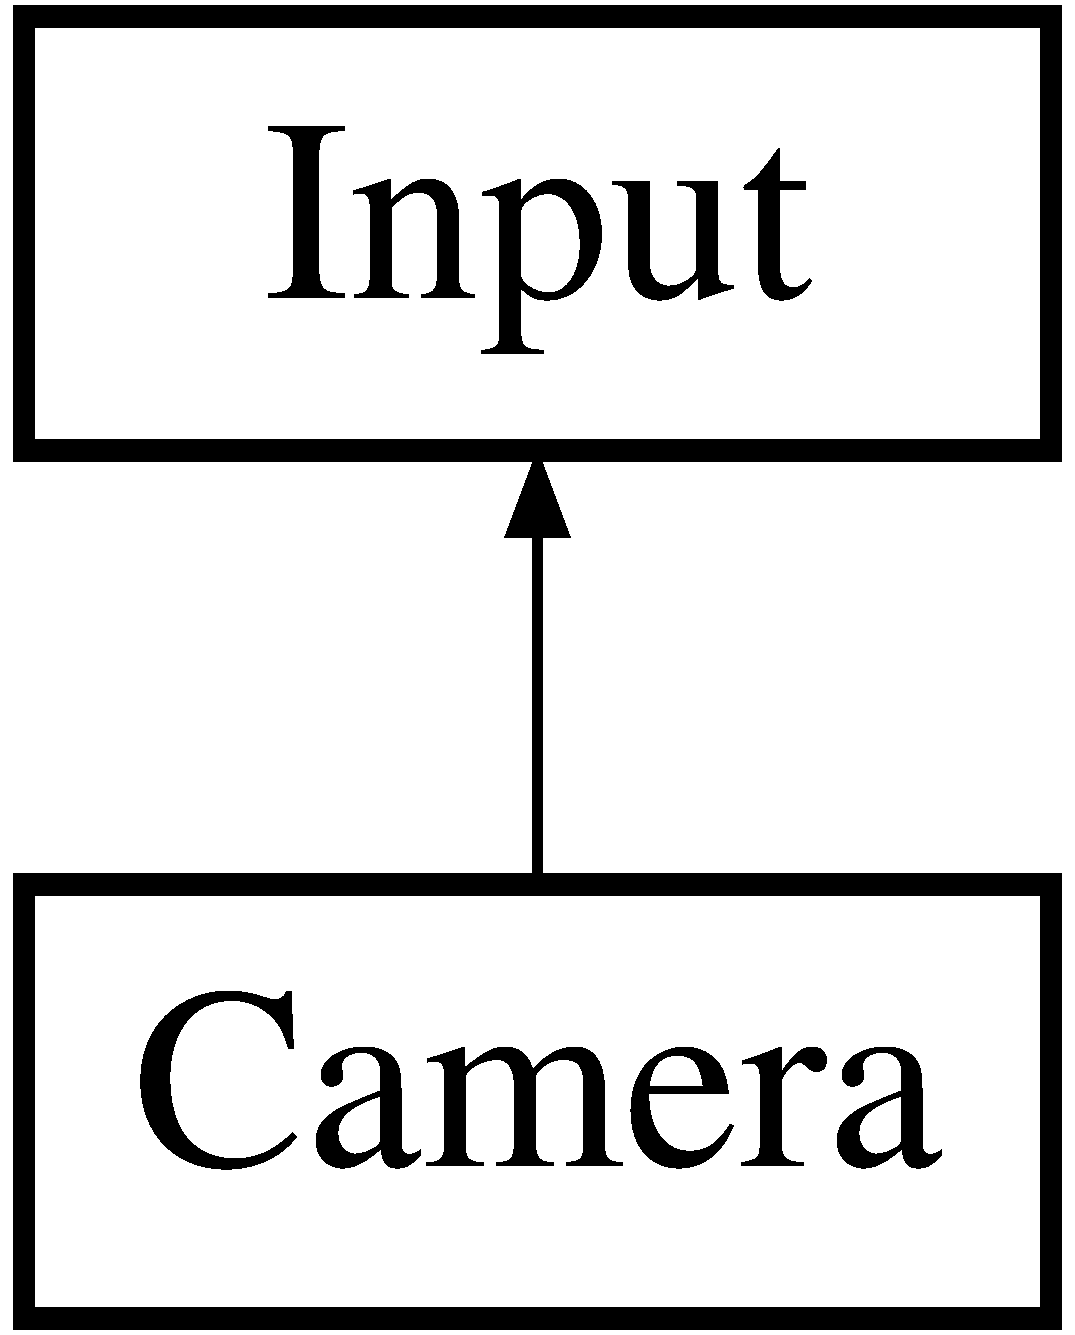
\includegraphics[height=2.000000cm]{class_input}
\end{center}
\end{figure}
\subsection*{Public Member Functions}
\begin{DoxyCompactItemize}
\item 
virtual void \hyperlink{class_input_a376e4472a9f3621238d6513252949366}{Handle\+Key} (unsigned char key, int state, int x, int y)
\item 
virtual void \hyperlink{class_input_adccce536f10dfe4b1de2bb22ed8ae538}{Handle\+Special\+Key} (int key, int state, int x, int y)
\item 
virtual void \hyperlink{class_input_a85fe43236eb168699ec57b37ab022741}{Handle\+Mouse} (int button, int state, int x, int y)
\item 
virtual void \hyperlink{class_input_abb590b1b9684b966340a8377ab0d00e2}{Handle\+Mouse\+Drag} (int x, int y)
\item 
virtual void \hyperlink{class_input_a89177666298fbef2797c677d486bc628}{Handle\+Mouse\+Move} (int x, int y)
\end{DoxyCompactItemize}


\subsection{Detailed Description}
Class for giving an coursework object input handling. Any class you want to have input handling should subclass the
\begin{DoxyCode}
\textcolor{keyword}{public} \hyperlink{class_input}{Input} 
\end{DoxyCode}
 . e.\+g.
\begin{DoxyCode}
MyObject : \textcolor{keyword}{public} \hyperlink{class_displayable_object}{DisplayableObject}, \textcolor{keyword}{public} \hyperlink{class_input}{Input} 
\end{DoxyCode}
 

Methods will be called from a \hyperlink{class_scene}{Scene} renderer to give input from keyboard and mouse \begin{DoxySeeAlso}{See also}
\hyperlink{class_camera}{Camera} 
\end{DoxySeeAlso}
\begin{DoxyAuthor}{Author}
wil 
\end{DoxyAuthor}


\subsection{Member Function Documentation}
\index{Input@{Input}!Handle\+Key@{Handle\+Key}}
\index{Handle\+Key@{Handle\+Key}!Input@{Input}}
\subsubsection[{\texorpdfstring{Handle\+Key(unsigned char key, int state, int x, int y)}{HandleKey(unsigned char key, int state, int x, int y)}}]{\setlength{\rightskip}{0pt plus 5cm}virtual void Input\+::\+Handle\+Key (
\begin{DoxyParamCaption}
\item[{unsigned char}]{key, }
\item[{int}]{state, }
\item[{int}]{x, }
\item[{int}]{y}
\end{DoxyParamCaption}
)\hspace{0.3cm}{\ttfamily [inline]}, {\ttfamily [virtual]}}\hypertarget{class_input_a376e4472a9f3621238d6513252949366}{}\label{class_input_a376e4472a9f3621238d6513252949366}
Called when keyboard input is received from A\+S\+C\+II characters. 

This includes keys E\+N\+T\+ER (\&\#92;n), R\+E\+T\+U\+RN (\&\#92;cr), T\+AB (\&\#92;t), B\+A\+C\+K\+S\+P\+A\+CE (\&\#92;b), E\+SC (27), D\+E\+L\+E\+TE (127) 

Note\+: check for R\+E\+T\+U\+RN and E\+N\+T\+ER for cross-\/platform operability. 

Example implementation\+: 
\begin{DoxyCode}
  \textcolor{keywordtype}{void} MyObject:\hyperlink{class_input_a376e4472a9f3621238d6513252949366}{HandleKey}(\textcolor{keywordtype}{unsigned} \textcolor{keywordtype}{char} key, \textcolor{keywordtype}{int} state, \textcolor{keywordtype}{int} mX, \textcolor{keywordtype}{int} mY)\{
      \textcolor{keywordflow}{if} (state == 1)\{ \textcolor{comment}{// if key pressed down}
        \textcolor{keywordflow}{switch}(key)\{ \textcolor{comment}{// ASCII char}
            \textcolor{keywordflow}{case} \textcolor{charliteral}{'A'}:
              \textcolor{keywordflow}{case} \textcolor{charliteral}{'a'}:
                  glTranslatef(-1.f,0.f,0.f); \textcolor{comment}{// go left}
                \textcolor{keywordflow}{break};
            \textcolor{keywordflow}{case} \textcolor{charliteral}{'D'}:
              \textcolor{keywordflow}{case} \textcolor{charliteral}{'d'}:
                  glTranslate(1.f,0.f,0.f); \textcolor{comment}{// go right}
                \textcolor{keywordflow}{break};
              \textcolor{keywordflow}{case} \textcolor{charliteral}{'\(\backslash\)n'}:  \textcolor{comment}{// Windows and Linux}
              \textcolor{keywordflow}{case} \textcolor{stringliteral}{'\(\backslash\)cr'}: \textcolor{comment}{// Mac OS X}
                  \textcolor{comment}{// operation for using enter/return key}
                \textcolor{keywordflow}{break};
        \}
    \}
\}
\end{DoxyCode}
 \begin{DoxySeeAlso}{See also}
\hyperlink{class_input_adccce536f10dfe4b1de2bb22ed8ae538}{Handle\+Special\+Key(int key, int state, int x, int y)} 
\end{DoxySeeAlso}

\begin{DoxyParams}{Parameters}
{\em key} & A\+S\+C\+II character from keyboard input \\
\hline
{\em state} & 1 if key down, 0 if key up \\
\hline
{\em x} & X coordinate of mouse in rendering window \\
\hline
{\em y} & Y coordinate of mouse in rendering window \\
\hline
\end{DoxyParams}


Reimplemented in \hyperlink{class_camera_aafed3cc6d06082a7396c38f4dd4a0549}{Camera}.

\index{Input@{Input}!Handle\+Mouse@{Handle\+Mouse}}
\index{Handle\+Mouse@{Handle\+Mouse}!Input@{Input}}
\subsubsection[{\texorpdfstring{Handle\+Mouse(int button, int state, int x, int y)}{HandleMouse(int button, int state, int x, int y)}}]{\setlength{\rightskip}{0pt plus 5cm}virtual void Input\+::\+Handle\+Mouse (
\begin{DoxyParamCaption}
\item[{int}]{button, }
\item[{int}]{state, }
\item[{int}]{x, }
\item[{int}]{y}
\end{DoxyParamCaption}
)\hspace{0.3cm}{\ttfamily [inline]}, {\ttfamily [virtual]}}\hypertarget{class_input_a85fe43236eb168699ec57b37ab022741}{}\label{class_input_a85fe43236eb168699ec57b37ab022741}
Called when mouse is clicked up / down in the rendering window 

button constants\+: G\+L\+U\+T\+\_\+\+L\+E\+F\+T\+\_\+\+B\+U\+T\+T\+ON, G\+L\+U\+T\+\_\+\+R\+I\+G\+H\+T\+\_\+\+B\+U\+T\+T\+ON and G\+L\+U\+T\+\_\+\+M\+I\+D\+D\+L\+E\+\_\+\+B\+U\+T\+T\+ON \begin{DoxySeeAlso}{See also}
\hyperlink{class_input_abb590b1b9684b966340a8377ab0d00e2}{Handle\+Mouse\+Drag(int x, int y)} 

\hyperlink{class_input_a89177666298fbef2797c677d486bc628}{Handle\+Mouse\+Move(int x, int y)} 
\end{DoxySeeAlso}

\begin{DoxyParams}{Parameters}
{\em button} & mouse button (G\+L\+U\+T\+\_\+\+L\+E\+F\+T\+\_\+\+B\+U\+T\+T\+ON, G\+L\+U\+T\+\_\+\+R\+I\+G\+H\+T\+\_\+\+B\+U\+T\+T\+ON or G\+L\+U\+T\+\_\+\+M\+I\+D\+D\+L\+E\+\_\+\+B\+U\+T\+T\+ON) \\
\hline
{\em state} & 1 if mouse down, 0 if mouse up \\
\hline
{\em x} & X coordinate of mouse in rendering window \\
\hline
{\em y} & Y coordinate of mouse in rendering window \\
\hline
\end{DoxyParams}


Reimplemented in \hyperlink{class_camera_adf8b8e5f8f1e88a373f102b3efa12697}{Camera}.

\index{Input@{Input}!Handle\+Mouse\+Drag@{Handle\+Mouse\+Drag}}
\index{Handle\+Mouse\+Drag@{Handle\+Mouse\+Drag}!Input@{Input}}
\subsubsection[{\texorpdfstring{Handle\+Mouse\+Drag(int x, int y)}{HandleMouseDrag(int x, int y)}}]{\setlength{\rightskip}{0pt plus 5cm}virtual void Input\+::\+Handle\+Mouse\+Drag (
\begin{DoxyParamCaption}
\item[{int}]{x, }
\item[{int}]{y}
\end{DoxyParamCaption}
)\hspace{0.3cm}{\ttfamily [inline]}, {\ttfamily [virtual]}}\hypertarget{class_input_abb590b1b9684b966340a8377ab0d00e2}{}\label{class_input_abb590b1b9684b966340a8377ab0d00e2}
Called when mouse is moved in rendering window while mouse button is held down \begin{DoxySeeAlso}{See also}
\hyperlink{class_input_a85fe43236eb168699ec57b37ab022741}{Handle\+Mouse(int button, int state, int x, int y)} 

\hyperlink{class_input_a89177666298fbef2797c677d486bc628}{Handle\+Mouse\+Move(int x, int y)} 
\end{DoxySeeAlso}

\begin{DoxyParams}{Parameters}
{\em x} & X coordinate of mouse in rendering window \\
\hline
{\em y} & Y coordinate of mouse in rendering window \\
\hline
\end{DoxyParams}


Reimplemented in \hyperlink{class_camera_af0b7923173a70a13f108ac69a8d9b848}{Camera}.

\index{Input@{Input}!Handle\+Mouse\+Move@{Handle\+Mouse\+Move}}
\index{Handle\+Mouse\+Move@{Handle\+Mouse\+Move}!Input@{Input}}
\subsubsection[{\texorpdfstring{Handle\+Mouse\+Move(int x, int y)}{HandleMouseMove(int x, int y)}}]{\setlength{\rightskip}{0pt plus 5cm}virtual void Input\+::\+Handle\+Mouse\+Move (
\begin{DoxyParamCaption}
\item[{int}]{x, }
\item[{int}]{y}
\end{DoxyParamCaption}
)\hspace{0.3cm}{\ttfamily [inline]}, {\ttfamily [virtual]}}\hypertarget{class_input_a89177666298fbef2797c677d486bc628}{}\label{class_input_a89177666298fbef2797c677d486bc628}
Called when mouse is moved in rendering window when no mouse button is pressed \begin{DoxySeeAlso}{See also}
\hyperlink{class_input_a85fe43236eb168699ec57b37ab022741}{Handle\+Mouse(int button, int state, int x, int y)} 

\hyperlink{class_input_abb590b1b9684b966340a8377ab0d00e2}{Handle\+Mouse\+Drag(int x, int y)} 
\end{DoxySeeAlso}

\begin{DoxyParams}{Parameters}
{\em x} & X coordinate of mouse in rendering window \\
\hline
{\em y} & Y coordinate of mouse in rendering window \\
\hline
\end{DoxyParams}


Reimplemented in \hyperlink{class_camera_a47357f68951777da13bef3234ff7474e}{Camera}.

\index{Input@{Input}!Handle\+Special\+Key@{Handle\+Special\+Key}}
\index{Handle\+Special\+Key@{Handle\+Special\+Key}!Input@{Input}}
\subsubsection[{\texorpdfstring{Handle\+Special\+Key(int key, int state, int x, int y)}{HandleSpecialKey(int key, int state, int x, int y)}}]{\setlength{\rightskip}{0pt plus 5cm}virtual void Input\+::\+Handle\+Special\+Key (
\begin{DoxyParamCaption}
\item[{int}]{key, }
\item[{int}]{state, }
\item[{int}]{x, }
\item[{int}]{y}
\end{DoxyParamCaption}
)\hspace{0.3cm}{\ttfamily [inline]}, {\ttfamily [virtual]}}\hypertarget{class_input_adccce536f10dfe4b1de2bb22ed8ae538}{}\label{class_input_adccce536f10dfe4b1de2bb22ed8ae538}
Called when keyboard input is received from special (non-\/\+A\+S\+C\+II) characters. 

key constants are named G\+L\+U\+T\+\_\+\+K\+E\+Y\+\_\+$\ast$ where $\ast$ is the key. For example\+: 

(arrow keys) G\+L\+U\+T\+\_\+\+K\+E\+Y\+\_\+\+UP, G\+L\+U\+T\+\_\+\+K\+E\+Y\+\_\+\+D\+O\+WN, G\+L\+U\+T\+\_\+\+K\+E\+Y\+\_\+\+L\+E\+FT, G\+L\+U\+T\+\_\+\+K\+E\+Y\+\_\+\+R\+I\+G\+HT, 

G\+L\+U\+T\+\_\+\+K\+E\+Y\+\_\+\+P\+A\+G\+E\+\_\+\+UP, G\+L\+U\+T\+\_\+\+K\+E\+Y\+\_\+\+P\+A\+G\+E\+\_\+\+D\+O\+WN, G\+L\+U\+T\+\_\+\+K\+E\+Y\+\_\+\+H\+O\+ME, G\+L\+U\+T\+\_\+\+K\+E\+Y\+\_\+\+E\+ND, 

G\+L\+U\+T\+\_\+\+K\+E\+Y\+\_\+\+F1, G\+L\+U\+T\+\_\+\+K\+E\+Y\+\_\+\+F2, etc. 

Example implementation\+: 
\begin{DoxyCode}
  \textcolor{keywordtype}{void} MyObject::HandleKey(\textcolor{keywordtype}{unsigned} \textcolor{keywordtype}{int} key, \textcolor{keywordtype}{int} state, \textcolor{keywordtype}{int} x, \textcolor{keywordtype}{int} y)\{
      \textcolor{keywordflow}{if} (state == 1)\{ \textcolor{comment}{// if key pressed down}
        \textcolor{keywordflow}{switch}(key)\{ \textcolor{comment}{// special key}
            \textcolor{keywordflow}{case} GLUT\_KEY\_LEFT:
                  glTranslate(-1.f,0.f,0.f); \textcolor{comment}{// go left}
                \textcolor{keywordflow}{break};
            \textcolor{keywordflow}{case} GLUT\_KEY\_RIGHT:
                  glTranslate(1.f,0.f,0.f); \textcolor{comment}{// go right}
                \textcolor{keywordflow}{break};
        \}
    \}
\}
\end{DoxyCode}
 \begin{DoxySeeAlso}{See also}
\#\+Handle\+Key(char key, int state, int x, int y) 
\end{DoxySeeAlso}

\begin{DoxyParams}{Parameters}
{\em key} & coded keyboard input \\
\hline
{\em state} & 1 if key down, 0 if key up \\
\hline
{\em x} & X coordinate of mouse in rendering window \\
\hline
{\em y} & Y coordinate of mouse in rendering window \\
\hline
\end{DoxyParams}


Reimplemented in \hyperlink{class_camera_aefce3308a5ed57fbc6666d8935fb7eac}{Camera}.



The documentation for this class was generated from the following file\+:\begin{DoxyCompactItemize}
\item 
Framework/\+Interface/Input.\+h\end{DoxyCompactItemize}

\hypertarget{class_my_scene}{}\section{My\+Scene Class Reference}
\label{class_my_scene}\index{My\+Scene@{My\+Scene}}
Inheritance diagram for My\+Scene\+:\begin{figure}[H]
\begin{center}
\leavevmode
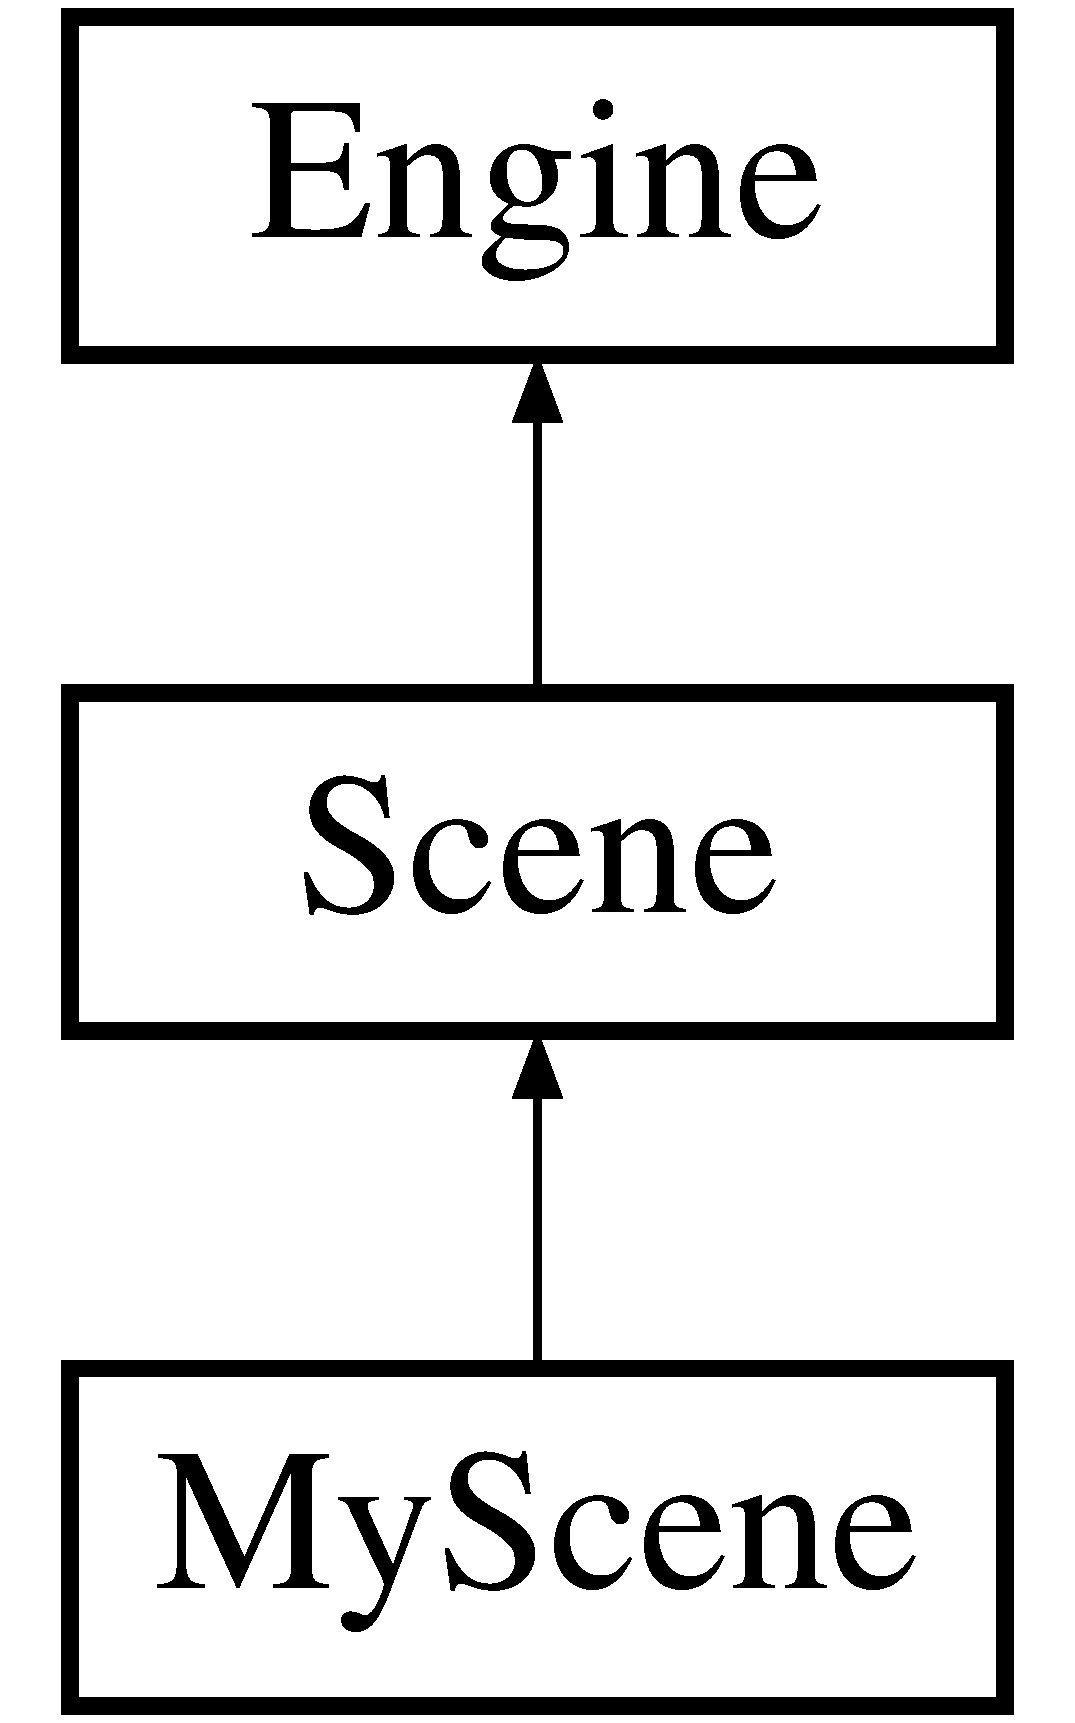
\includegraphics[height=3.000000cm]{class_my_scene}
\end{center}
\end{figure}
\subsection*{Public Member Functions}
\begin{DoxyCompactItemize}
\item 
{\bfseries My\+Scene} (int argc, char $\ast$$\ast$argv, const char $\ast$title, const int \&window\+Width, const int \&window\+Height)\hypertarget{class_my_scene_ac1ab21722818b5d7102cf5174f0cc4c5}{}\label{class_my_scene_ac1ab21722818b5d7102cf5174f0cc4c5}

\end{DoxyCompactItemize}
\subsection*{Additional Inherited Members}


The documentation for this class was generated from the following files\+:\begin{DoxyCompactItemize}
\item 
Code/My\+Scene.\+h\item 
Code/My\+Scene.\+cpp\end{DoxyCompactItemize}

\hypertarget{class_scene}{}\section{Scene Class Reference}
\label{class_scene}\index{Scene@{Scene}}
Inheritance diagram for Scene\+:\begin{figure}[H]
\begin{center}
\leavevmode
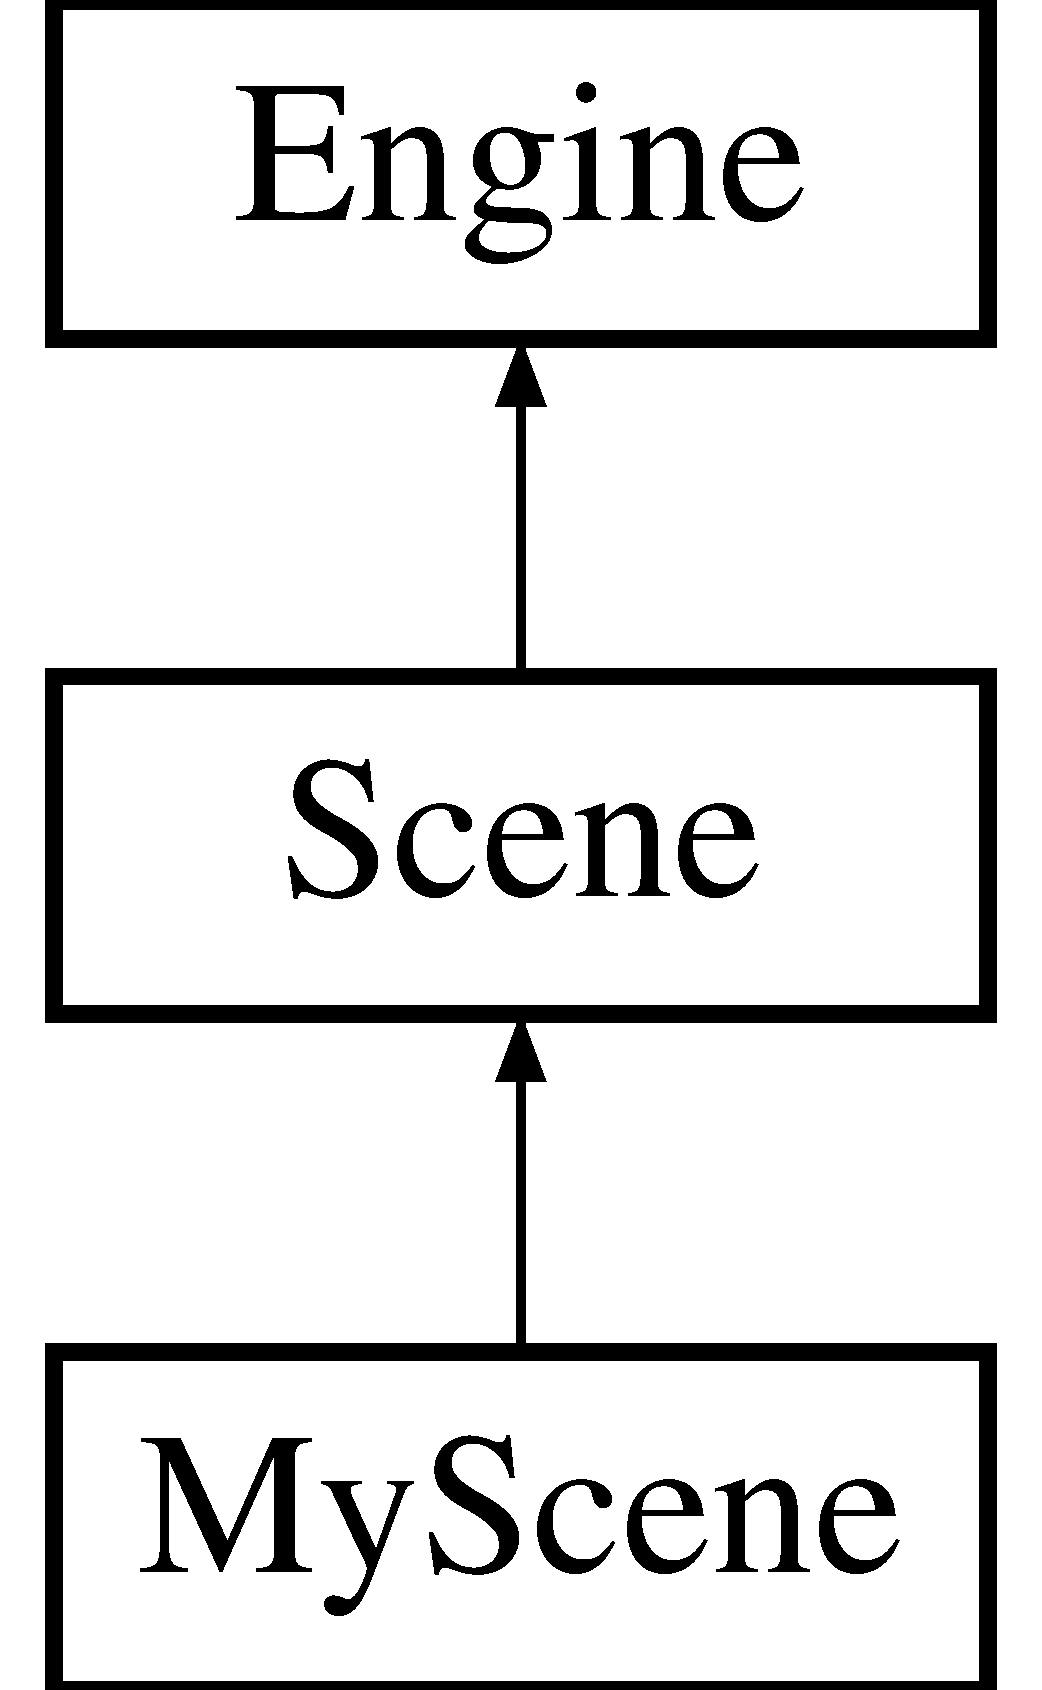
\includegraphics[height=3.000000cm]{class_scene}
\end{center}
\end{figure}
\subsection*{Public Member Functions}
\begin{DoxyCompactItemize}
\item 
\hyperlink{class_scene_a75a2d7229276dfb590272846083cc64d}{Scene} (int argc, char $\ast$$\ast$argv, const char $\ast$title, const int \&window\+Width, const int \&window\+Height)
\item 
virtual \hyperlink{class_scene_a3b8cec2e32546713915f8c6303c951f1}{$\sim$\+Scene} ()
\end{DoxyCompactItemize}
\subsection*{Static Public Member Functions}
\begin{DoxyCompactItemize}
\item 
static int \hyperlink{class_scene_ac311bf97401b0d26e6df07efed35d355}{Get\+Window\+Width} ()
\item 
static int \hyperlink{class_scene_a178707699459f782a39ed7f6508ccd41}{Get\+Window\+Height} ()
\item 
static int \hyperlink{class_scene_ad2ff858bbd74d760d543bb29ca8c8153}{Get\+Texture} (std\+::string file\+Name)
\item 
static \hyperlink{class_camera}{Camera} $\ast$ \hyperlink{class_scene_aa08b6b22037aa939e6e6fe732765bc66}{Get\+Camera} ()
\end{DoxyCompactItemize}
\subsection*{Protected Member Functions}
\begin{DoxyCompactItemize}
\item 
virtual void \hyperlink{class_scene_ac97910ce8ed0aa0498a796d1cc7e0df5}{Initialise} ()=0
\item 
void \hyperlink{class_scene_a4813338ee7c6c995f5bb6f10e3673804}{Draw} ()
\item 
void \hyperlink{class_scene_a66107de97484c0f9a060e008cdc7320b}{Reshape} (int w, int h)
\item 
virtual void \hyperlink{class_scene_a6bf51e06c437c820c848be4c76c5ddae}{Projection} ()
\item 
void \hyperlink{class_scene_ab18f75e30620503fbfe2fb138116be5b}{Update} (const double \&delta\+Time)
\item 
void {\bfseries Handle\+Key} (unsigned char key, int state, int x, int y)\hypertarget{class_scene_a869ee0cb7f2b96b15ba6a7cce7e8358a}{}\label{class_scene_a869ee0cb7f2b96b15ba6a7cce7e8358a}

\item 
void {\bfseries Handle\+Special\+Key} (int key, int state, int x, int y)\hypertarget{class_scene_a8d878c181721d6dceac001de0ee73810}{}\label{class_scene_a8d878c181721d6dceac001de0ee73810}

\item 
void {\bfseries Handle\+Mouse} (int button, int state, int x, int y)\hypertarget{class_scene_a523a91aec3a7f546356dd0a06eb1d563}{}\label{class_scene_a523a91aec3a7f546356dd0a06eb1d563}

\item 
void {\bfseries Handle\+Mouse\+Drag} (int x, int y)\hypertarget{class_scene_a2265ef3985ed79dfa7f942b615fab3eb}{}\label{class_scene_a2265ef3985ed79dfa7f942b615fab3eb}

\item 
void {\bfseries Handle\+Mouse\+Move} (int x, int y)\hypertarget{class_scene_a43334d6db1ff83d24135aa566c318b6d}{}\label{class_scene_a43334d6db1ff83d24135aa566c318b6d}

\item 
void \hyperlink{class_scene_ab42e4830fe5baac28fa3e6d144492a82}{Add\+Object\+To\+Scene} (\hyperlink{class_displayable_object}{Displayable\+Object} $\ast$obj)
\end{DoxyCompactItemize}
\subsection*{Additional Inherited Members}


\subsection{Constructor \& Destructor Documentation}
\index{Scene@{Scene}!Scene@{Scene}}
\index{Scene@{Scene}!Scene@{Scene}}
\subsubsection[{\texorpdfstring{Scene(int argc, char $\ast$$\ast$argv, const char $\ast$title, const int \&window\+Width, const int \&window\+Height)}{Scene(int argc, char **argv, const char *title, const int &windowWidth, const int &windowHeight)}}]{\setlength{\rightskip}{0pt plus 5cm}Scene\+::\+Scene (
\begin{DoxyParamCaption}
\item[{int}]{argc, }
\item[{char $\ast$$\ast$}]{argv, }
\item[{const char $\ast$}]{title, }
\item[{const int \&}]{window\+Width, }
\item[{const int \&}]{window\+Height}
\end{DoxyParamCaption}
)}\hypertarget{class_scene_a75a2d7229276dfb590272846083cc64d}{}\label{class_scene_a75a2d7229276dfb590272846083cc64d}
Constructor, overrides \hyperlink{class_engine_a06d6fce9529416545e9b88edf5128358}{Engine()} and takes in command line arguments, a title and initial window dimensions. \index{Scene@{Scene}!````~Scene@{$\sim$\+Scene}}
\index{````~Scene@{$\sim$\+Scene}!Scene@{Scene}}
\subsubsection[{\texorpdfstring{$\sim$\+Scene()}{~Scene()}}]{\setlength{\rightskip}{0pt plus 5cm}Scene\+::$\sim$\+Scene (
\begin{DoxyParamCaption}
{}
\end{DoxyParamCaption}
)\hspace{0.3cm}{\ttfamily [virtual]}}\hypertarget{class_scene_a3b8cec2e32546713915f8c6303c951f1}{}\label{class_scene_a3b8cec2e32546713915f8c6303c951f1}
Destructor\+: deletes all \hyperlink{class_displayable_object}{Displayable\+Object}s in the \hyperlink{class_scene}{Scene} 

\subsection{Member Function Documentation}
\index{Scene@{Scene}!Add\+Object\+To\+Scene@{Add\+Object\+To\+Scene}}
\index{Add\+Object\+To\+Scene@{Add\+Object\+To\+Scene}!Scene@{Scene}}
\subsubsection[{\texorpdfstring{Add\+Object\+To\+Scene(\+Displayable\+Object $\ast$obj)}{AddObjectToScene(DisplayableObject *obj)}}]{\setlength{\rightskip}{0pt plus 5cm}void Scene\+::\+Add\+Object\+To\+Scene (
\begin{DoxyParamCaption}
\item[{{\bf Displayable\+Object} $\ast$}]{obj}
\end{DoxyParamCaption}
)\hspace{0.3cm}{\ttfamily [protected]}}\hypertarget{class_scene_ab42e4830fe5baac28fa3e6d144492a82}{}\label{class_scene_ab42e4830fe5baac28fa3e6d144492a82}
Adds a \hyperlink{class_displayable_object}{Displayable\+Object} (includes \hyperlink{class_animation}{Animation}s) to the \hyperlink{class_scene}{Scene}. 

It is strongly recommended you do N\+OT attempt to override this method. \begin{DoxySeeAlso}{See also}
\#add\+Object\+To\+Scene(\+Displayable\+Object, String) 

\#get\+Object(\+String) 
\end{DoxySeeAlso}

\begin{DoxyParams}{Parameters}
{\em obj} & \hyperlink{class_displayable_object}{Displayable\+Object} to be added to the scene. \\
\hline
\end{DoxyParams}
\index{Scene@{Scene}!Draw@{Draw}}
\index{Draw@{Draw}!Scene@{Scene}}
\subsubsection[{\texorpdfstring{Draw()}{Draw()}}]{\setlength{\rightskip}{0pt plus 5cm}void Scene\+::\+Draw (
\begin{DoxyParamCaption}
{}
\end{DoxyParamCaption}
)\hspace{0.3cm}{\ttfamily [protected]}, {\ttfamily [virtual]}}\hypertarget{class_scene_a4813338ee7c6c995f5bb6f10e3673804}{}\label{class_scene_a4813338ee7c6c995f5bb6f10e3673804}
This function will loop continuously until the program is exited. It will iterate through the objects and render in your \hyperlink{class_scene}{Scene} 

The frequency at which
\begin{DoxyCode}
\hyperlink{class_scene_a4813338ee7c6c995f5bb6f10e3673804}{Draw}() 
\end{DoxyCode}
 is called per second is dependent on your hardware and scene, so for animation, you M\+U\+ST use the \hyperlink{class_scene_ab18f75e30620503fbfe2fb138116be5b}{Update} method with
\begin{DoxyCode}
deltaTime 
\end{DoxyCode}
 

It is strongly recommended you do N\+OT attempt to override this method. 


\begin{DoxyCode}
\hyperlink{class_scene_a4813338ee7c6c995f5bb6f10e3673804}{Draw}() 
\end{DoxyCode}
 should N\+E\+V\+ER be called explicitly. \begin{DoxySeeAlso}{See also}
\hyperlink{class_scene_a66107de97484c0f9a060e008cdc7320b}{Reshape()} 
\end{DoxySeeAlso}


Implements \hyperlink{class_engine}{Engine}.

\index{Scene@{Scene}!Get\+Camera@{Get\+Camera}}
\index{Get\+Camera@{Get\+Camera}!Scene@{Scene}}
\subsubsection[{\texorpdfstring{Get\+Camera()}{GetCamera()}}]{\setlength{\rightskip}{0pt plus 5cm}static {\bf Camera}$\ast$ Scene\+::\+Get\+Camera (
\begin{DoxyParamCaption}
{}
\end{DoxyParamCaption}
)\hspace{0.3cm}{\ttfamily [inline]}, {\ttfamily [static]}}\hypertarget{class_scene_aa08b6b22037aa939e6e6fe732765bc66}{}\label{class_scene_aa08b6b22037aa939e6e6fe732765bc66}
Returns a pointer to the \hyperlink{class_camera}{Camera} \index{Scene@{Scene}!Get\+Texture@{Get\+Texture}}
\index{Get\+Texture@{Get\+Texture}!Scene@{Scene}}
\subsubsection[{\texorpdfstring{Get\+Texture(std\+::string file\+Name)}{GetTexture(std::string fileName)}}]{\setlength{\rightskip}{0pt plus 5cm}int Scene\+::\+Get\+Texture (
\begin{DoxyParamCaption}
\item[{std\+::string}]{file\+Name}
\end{DoxyParamCaption}
)\hspace{0.3cm}{\ttfamily [static]}}\hypertarget{class_scene_ad2ff858bbd74d760d543bb29ca8c8153}{}\label{class_scene_ad2ff858bbd74d760d543bb29ca8c8153}
\hyperlink{class_input}{Input} a .bmp bitmap image to bind to internal texture buffer \begin{DoxyReturn}{Returns}
texture\+ID  file\+Name the name of the texture file you want to input 
\end{DoxyReturn}
\index{Scene@{Scene}!Get\+Window\+Height@{Get\+Window\+Height}}
\index{Get\+Window\+Height@{Get\+Window\+Height}!Scene@{Scene}}
\subsubsection[{\texorpdfstring{Get\+Window\+Height()}{GetWindowHeight()}}]{\setlength{\rightskip}{0pt plus 5cm}int Scene\+::\+Get\+Window\+Height (
\begin{DoxyParamCaption}
{}
\end{DoxyParamCaption}
)\hspace{0.3cm}{\ttfamily [static]}}\hypertarget{class_scene_a178707699459f782a39ed7f6508ccd41}{}\label{class_scene_a178707699459f782a39ed7f6508ccd41}
Return window height \index{Scene@{Scene}!Get\+Window\+Width@{Get\+Window\+Width}}
\index{Get\+Window\+Width@{Get\+Window\+Width}!Scene@{Scene}}
\subsubsection[{\texorpdfstring{Get\+Window\+Width()}{GetWindowWidth()}}]{\setlength{\rightskip}{0pt plus 5cm}int Scene\+::\+Get\+Window\+Width (
\begin{DoxyParamCaption}
{}
\end{DoxyParamCaption}
)\hspace{0.3cm}{\ttfamily [static]}}\hypertarget{class_scene_ac311bf97401b0d26e6df07efed35d355}{}\label{class_scene_ac311bf97401b0d26e6df07efed35d355}
Return window width \index{Scene@{Scene}!Initialise@{Initialise}}
\index{Initialise@{Initialise}!Scene@{Scene}}
\subsubsection[{\texorpdfstring{Initialise()=0}{Initialise()=0}}]{\setlength{\rightskip}{0pt plus 5cm}void Scene\+::\+Initialise (
\begin{DoxyParamCaption}
{}
\end{DoxyParamCaption}
)\hspace{0.3cm}{\ttfamily [protected]}, {\ttfamily [pure virtual]}}\hypertarget{class_scene_ac97910ce8ed0aa0498a796d1cc7e0df5}{}\label{class_scene_ac97910ce8ed0aa0498a796d1cc7e0df5}
This must be overloaded this to add \hyperlink{class_displayable_object}{Displayable\+Object}s to your scene. \begin{DoxySeeAlso}{See also}
\hyperlink{class_scene_a6bf51e06c437c820c848be4c76c5ddae}{Projection()} 
\end{DoxySeeAlso}


Implements \hyperlink{class_engine}{Engine}.

\index{Scene@{Scene}!Projection@{Projection}}
\index{Projection@{Projection}!Scene@{Scene}}
\subsubsection[{\texorpdfstring{Projection()}{Projection()}}]{\setlength{\rightskip}{0pt plus 5cm}void Scene\+::\+Projection (
\begin{DoxyParamCaption}
{}
\end{DoxyParamCaption}
)\hspace{0.3cm}{\ttfamily [protected]}, {\ttfamily [virtual]}}\hypertarget{class_scene_a6bf51e06c437c820c848be4c76c5ddae}{}\label{class_scene_a6bf51e06c437c820c848be4c76c5ddae}
Sets the projection properties of the scene. Override to change projection properties. 

Default\+: Orthographic mode \index{Scene@{Scene}!Reshape@{Reshape}}
\index{Reshape@{Reshape}!Scene@{Scene}}
\subsubsection[{\texorpdfstring{Reshape(int w, int h)}{Reshape(int w, int h)}}]{\setlength{\rightskip}{0pt plus 5cm}void Scene\+::\+Reshape (
\begin{DoxyParamCaption}
\item[{int}]{w, }
\item[{int}]{h}
\end{DoxyParamCaption}
)\hspace{0.3cm}{\ttfamily [protected]}, {\ttfamily [virtual]}}\hypertarget{class_scene_a66107de97484c0f9a060e008cdc7320b}{}\label{class_scene_a66107de97484c0f9a060e008cdc7320b}
Called when the window is resized, and handles resizing events. 

You should this function to handle the window being resized. The default property is to update the projection parameters. You can access the window size parameters by the
\begin{DoxyCode}
w 
\end{DoxyCode}
 and
\begin{DoxyCode}
h 
\end{DoxyCode}
 variables. For example, you could overload this function to adjust the size of all objects in your
\begin{DoxyCode}
\hyperlink{class_scene}{Scene} 
\end{DoxyCode}
 . \begin{DoxySeeAlso}{See also}
\hyperlink{class_scene_a4813338ee7c6c995f5bb6f10e3673804}{Draw()} 

\hyperlink{class_scene_a6bf51e06c437c820c848be4c76c5ddae}{Projection()} 

\hyperlink{class_scene_ac97910ce8ed0aa0498a796d1cc7e0df5}{Initialise()} 
\end{DoxySeeAlso}


Implements \hyperlink{class_engine}{Engine}.

\index{Scene@{Scene}!Update@{Update}}
\index{Update@{Update}!Scene@{Scene}}
\subsubsection[{\texorpdfstring{Update(const double \&delta\+Time)}{Update(const double &deltaTime)}}]{\setlength{\rightskip}{0pt plus 5cm}void Scene\+::\+Update (
\begin{DoxyParamCaption}
\item[{const double \&}]{delta\+Time}
\end{DoxyParamCaption}
)\hspace{0.3cm}{\ttfamily [protected]}, {\ttfamily [virtual]}}\hypertarget{class_scene_ab18f75e30620503fbfe2fb138116be5b}{}\label{class_scene_ab18f75e30620503fbfe2fb138116be5b}
The update function for \hyperlink{class_camera}{Camera} and \hyperlink{class_animation}{Animation}. Calculates the time-\/delay since the last update and passes as a parameter to the respective class\textquotesingle{}s
\begin{DoxyCode}
\hyperlink{class_scene_ab18f75e30620503fbfe2fb138116be5b}{Update}() 
\end{DoxyCode}
 functions. 

You should only override this class if you want to change how the animation update function works. This is not advised. \begin{DoxySeeAlso}{See also}
\hyperlink{class_camera}{Camera} 

\hyperlink{class_animation}{Animation} 

\hyperlink{class_scene_a4813338ee7c6c995f5bb6f10e3673804}{Draw()} 
\end{DoxySeeAlso}


Implements \hyperlink{class_engine}{Engine}.



The documentation for this class was generated from the following files\+:\begin{DoxyCompactItemize}
\item 
Framework/\+Engine/Scene.\+h\item 
Framework/\+Engine/Scene.\+cpp\end{DoxyCompactItemize}

\hypertarget{structtag_b_i_t_m_a_p_f_i_l_e_h_e_a_d_e_r}{}\section{tag\+B\+I\+T\+M\+A\+P\+F\+I\+L\+E\+H\+E\+A\+D\+ER Struct Reference}
\label{structtag_b_i_t_m_a_p_f_i_l_e_h_e_a_d_e_r}\index{tag\+B\+I\+T\+M\+A\+P\+F\+I\+L\+E\+H\+E\+A\+D\+ER@{tag\+B\+I\+T\+M\+A\+P\+F\+I\+L\+E\+H\+E\+A\+D\+ER}}
\subsection*{Public Attributes}
\begin{DoxyCompactItemize}
\item 
W\+O\+RD {\bfseries bf\+Type}\hypertarget{structtag_b_i_t_m_a_p_f_i_l_e_h_e_a_d_e_r_a64ced0b35fb93012ce3d66b2f1dd5bb8}{}\label{structtag_b_i_t_m_a_p_f_i_l_e_h_e_a_d_e_r_a64ced0b35fb93012ce3d66b2f1dd5bb8}

\item 
D\+W\+O\+RD {\bfseries bf\+Size}\hypertarget{structtag_b_i_t_m_a_p_f_i_l_e_h_e_a_d_e_r_ad6fa0d3a907934d597b2773bc45e4d43}{}\label{structtag_b_i_t_m_a_p_f_i_l_e_h_e_a_d_e_r_ad6fa0d3a907934d597b2773bc45e4d43}

\item 
W\+O\+RD {\bfseries bf\+Reserved1}\hypertarget{structtag_b_i_t_m_a_p_f_i_l_e_h_e_a_d_e_r_aee794445cde1ce265644c1718afc6b52}{}\label{structtag_b_i_t_m_a_p_f_i_l_e_h_e_a_d_e_r_aee794445cde1ce265644c1718afc6b52}

\item 
W\+O\+RD {\bfseries bf\+Reserved2}\hypertarget{structtag_b_i_t_m_a_p_f_i_l_e_h_e_a_d_e_r_a017d814d24a7c65de297be31856501dc}{}\label{structtag_b_i_t_m_a_p_f_i_l_e_h_e_a_d_e_r_a017d814d24a7c65de297be31856501dc}

\item 
D\+W\+O\+RD {\bfseries bf\+Off\+Bits}\hypertarget{structtag_b_i_t_m_a_p_f_i_l_e_h_e_a_d_e_r_a5740a971a88afb51b014f54d9eb1c95c}{}\label{structtag_b_i_t_m_a_p_f_i_l_e_h_e_a_d_e_r_a5740a971a88afb51b014f54d9eb1c95c}

\end{DoxyCompactItemize}


The documentation for this struct was generated from the following file\+:\begin{DoxyCompactItemize}
\item 
Framework/\+Utility/Texture.\+cpp\end{DoxyCompactItemize}

\hypertarget{structtag_b_i_t_m_a_p_i_n_f_o_h_e_a_d_e_r}{}\section{tag\+B\+I\+T\+M\+A\+P\+I\+N\+F\+O\+H\+E\+A\+D\+ER Struct Reference}
\label{structtag_b_i_t_m_a_p_i_n_f_o_h_e_a_d_e_r}\index{tag\+B\+I\+T\+M\+A\+P\+I\+N\+F\+O\+H\+E\+A\+D\+ER@{tag\+B\+I\+T\+M\+A\+P\+I\+N\+F\+O\+H\+E\+A\+D\+ER}}
\subsection*{Public Attributes}
\begin{DoxyCompactItemize}
\item 
D\+W\+O\+RD {\bfseries bi\+Size}\hypertarget{structtag_b_i_t_m_a_p_i_n_f_o_h_e_a_d_e_r_a78b47f256953606cbf23cd665452a263}{}\label{structtag_b_i_t_m_a_p_i_n_f_o_h_e_a_d_e_r_a78b47f256953606cbf23cd665452a263}

\item 
L\+O\+NG {\bfseries bi\+Width}\hypertarget{structtag_b_i_t_m_a_p_i_n_f_o_h_e_a_d_e_r_a4bbc605184be98c4da36f707f7695e0f}{}\label{structtag_b_i_t_m_a_p_i_n_f_o_h_e_a_d_e_r_a4bbc605184be98c4da36f707f7695e0f}

\item 
L\+O\+NG {\bfseries bi\+Height}\hypertarget{structtag_b_i_t_m_a_p_i_n_f_o_h_e_a_d_e_r_aa18cf290b7f7a6d1cc8058feae85ab68}{}\label{structtag_b_i_t_m_a_p_i_n_f_o_h_e_a_d_e_r_aa18cf290b7f7a6d1cc8058feae85ab68}

\item 
W\+O\+RD {\bfseries bi\+Planes}\hypertarget{structtag_b_i_t_m_a_p_i_n_f_o_h_e_a_d_e_r_a261e0f0a578bcd4d53a4a221e6ebe2fa}{}\label{structtag_b_i_t_m_a_p_i_n_f_o_h_e_a_d_e_r_a261e0f0a578bcd4d53a4a221e6ebe2fa}

\item 
W\+O\+RD {\bfseries bi\+Bit\+Count}\hypertarget{structtag_b_i_t_m_a_p_i_n_f_o_h_e_a_d_e_r_a713c58f9cf7d5f115938d189d59fadf5}{}\label{structtag_b_i_t_m_a_p_i_n_f_o_h_e_a_d_e_r_a713c58f9cf7d5f115938d189d59fadf5}

\item 
D\+W\+O\+RD {\bfseries bi\+Compression}\hypertarget{structtag_b_i_t_m_a_p_i_n_f_o_h_e_a_d_e_r_a6b50d93eae77d44af8907740e337583d}{}\label{structtag_b_i_t_m_a_p_i_n_f_o_h_e_a_d_e_r_a6b50d93eae77d44af8907740e337583d}

\item 
D\+W\+O\+RD {\bfseries bi\+Size\+Image}\hypertarget{structtag_b_i_t_m_a_p_i_n_f_o_h_e_a_d_e_r_ac69dfda61a32d8ec53dd11ef165d198b}{}\label{structtag_b_i_t_m_a_p_i_n_f_o_h_e_a_d_e_r_ac69dfda61a32d8ec53dd11ef165d198b}

\item 
L\+O\+NG {\bfseries bi\+X\+Pels\+Per\+Meter}\hypertarget{structtag_b_i_t_m_a_p_i_n_f_o_h_e_a_d_e_r_ae363738b6e92248a7be41f4e7ed55c54}{}\label{structtag_b_i_t_m_a_p_i_n_f_o_h_e_a_d_e_r_ae363738b6e92248a7be41f4e7ed55c54}

\item 
L\+O\+NG {\bfseries bi\+Y\+Pels\+Per\+Meter}\hypertarget{structtag_b_i_t_m_a_p_i_n_f_o_h_e_a_d_e_r_ac6226594275d045ff0d03849945d920f}{}\label{structtag_b_i_t_m_a_p_i_n_f_o_h_e_a_d_e_r_ac6226594275d045ff0d03849945d920f}

\item 
D\+W\+O\+RD {\bfseries bi\+Clr\+Used}\hypertarget{structtag_b_i_t_m_a_p_i_n_f_o_h_e_a_d_e_r_adbf6bd52839895672030a734d2ae752f}{}\label{structtag_b_i_t_m_a_p_i_n_f_o_h_e_a_d_e_r_adbf6bd52839895672030a734d2ae752f}

\item 
D\+W\+O\+RD {\bfseries bi\+Clr\+Important}\hypertarget{structtag_b_i_t_m_a_p_i_n_f_o_h_e_a_d_e_r_a637282b108fc8ac3bdf41479f9931ccb}{}\label{structtag_b_i_t_m_a_p_i_n_f_o_h_e_a_d_e_r_a637282b108fc8ac3bdf41479f9931ccb}

\end{DoxyCompactItemize}


The documentation for this struct was generated from the following file\+:\begin{DoxyCompactItemize}
\item 
Framework/\+Utility/Texture.\+cpp\end{DoxyCompactItemize}

\hypertarget{class_texture}{}\section{Texture Class Reference}
\label{class_texture}\index{Texture@{Texture}}


{\ttfamily \#include $<$Texture.\+h$>$}

\subsection*{Public Member Functions}
\begin{DoxyCompactItemize}
\item 
int \hyperlink{class_texture_a5d20fa1d3eb2483eb9744f92ae83be03}{Get\+Texture} (std\+::string file\+Name)
\end{DoxyCompactItemize}


\subsection{Detailed Description}
Class for loading bitmap files into texture buffer and handling texture I\+Ds 

\subsection{Member Function Documentation}
\index{Texture@{Texture}!Get\+Texture@{Get\+Texture}}
\index{Get\+Texture@{Get\+Texture}!Texture@{Texture}}
\subsubsection[{\texorpdfstring{Get\+Texture(std\+::string file\+Name)}{GetTexture(std::string fileName)}}]{\setlength{\rightskip}{0pt plus 5cm}int Texture\+::\+Get\+Texture (
\begin{DoxyParamCaption}
\item[{std\+::string}]{file\+Name}
\end{DoxyParamCaption}
)}\hypertarget{class_texture_a5d20fa1d3eb2483eb9744f92ae83be03}{}\label{class_texture_a5d20fa1d3eb2483eb9744f92ae83be03}
Loads a texture into memory and returns the id of the texture object created 

The documentation for this class was generated from the following files\+:\begin{DoxyCompactItemize}
\item 
Framework/\+Utility/Texture.\+h\item 
Framework/\+Utility/Texture.\+cpp\end{DoxyCompactItemize}

%--- End generated contents ---

% Index
\backmatter
\newpage
\phantomsection
\clearemptydoublepage
\addcontentsline{toc}{chapter}{Index}
\printindex

\end{document}
